\subsection{NuMI as a Sideband/Elena}
MicroBooNE is exposed to an orthogonal, sizable source of neutrinos which can be used as sideband to cross check BNB $\nu_e$ searches: the NuMI beam.  Albeit the energy of the protons generating the NuMI beam is much higher (120 GeV compared to the usual 8 GeV of the Booster),  neutrinos from NuMI cover an energy range similar to the neutrinos from BNB, because of the highly off-axis nature of the NuMI beam at MicroBooNE. Additionally, the electron $\nu_e$ and $\bar\nu_e$ content of the beam is about an order of magnitude higher in NuMI compared to the instrinsic $\nu_e$ BNB prediction.  
Oscillation effects in NuMI are predicted to be small and extremely difficult to disentangle from the flux predictions for the intrinsic electron neutrinos. Details on the NuMI beam characteristics and flux predictions can be found in Ref.~\cite{bib:NuMIFlux}.

\subsubsection{Overview of NuMI data set}
The availability of NuMI data has been limited. Thus, the results presented in this section are obtained only with a Run 1 sample of 8.885e19 POT on beam and $\sim$4M EXT triggers (both corresponding to about half of the  Run 1 collected sample), as well as simulated $\nu$ overlay and dirt samples corresponding to 2.071e21 POT  and 1.421e21 POT, respectively. The result presented only show statistical uncertainty, not considering cross section or flux systematics. We follow the current best practices for NuMI POT normalization in MCC9, which entail a reduction of the NuMI EXT trigger by 2\% (to account for neutrino trigger occupancy) and a reduction of the dirt by 65\% (constraint using the event flash timing); more details on the NuMI POT normalization can be found in \cite{bib:NuMINorm}. 


\subsubsection{NuMI 1eNp Sideband/Elena}
Figure~\ref{fig:NuMI_1eNp_reco_e} shows the reconstructed energy spectrum for \npsel after the final \npsel selection using the currently available 8.885e19  POT from Run 1 NuMI data.

\begin{figure}[H]
    \begin{center}
    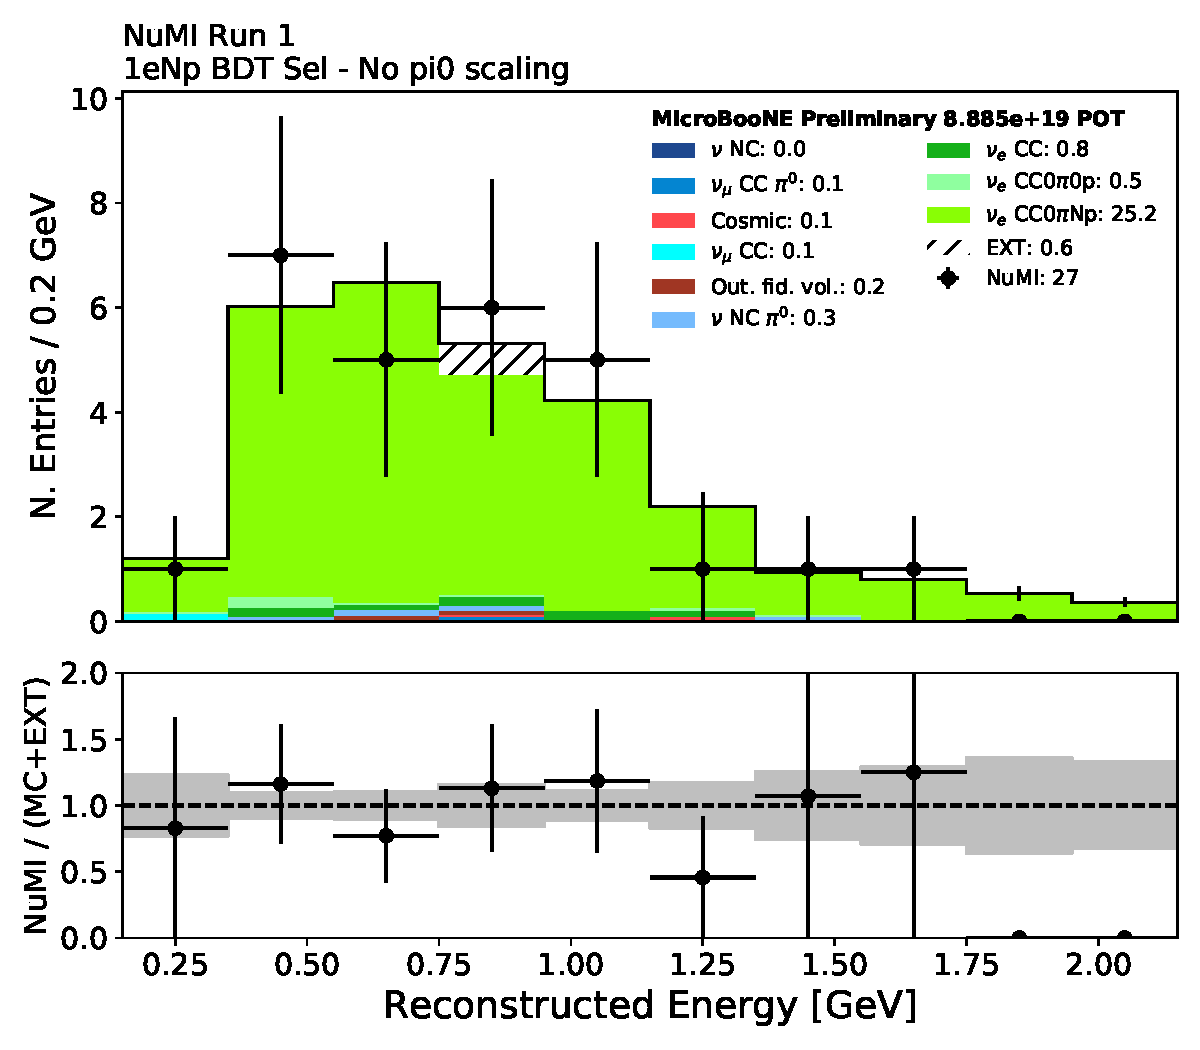
\includegraphics[width=0.5\textwidth]{Sidebands/Figures/NuMI/1eNp/BDTSel/reco_e.pdf}
    \caption{}
    \label{fig:NuMI_1eNp_reco_e}
    \end{center}
\end{figure}



Figures~\ref{fig:NuMI_1eNp_1} to~\ref{fig:NuMI_1eNp_5} show all BDT input variables from the   loose selection stage.

\begin{figure}[H]
    \centering
    \begin{subfigure}{0.3\textwidth}
    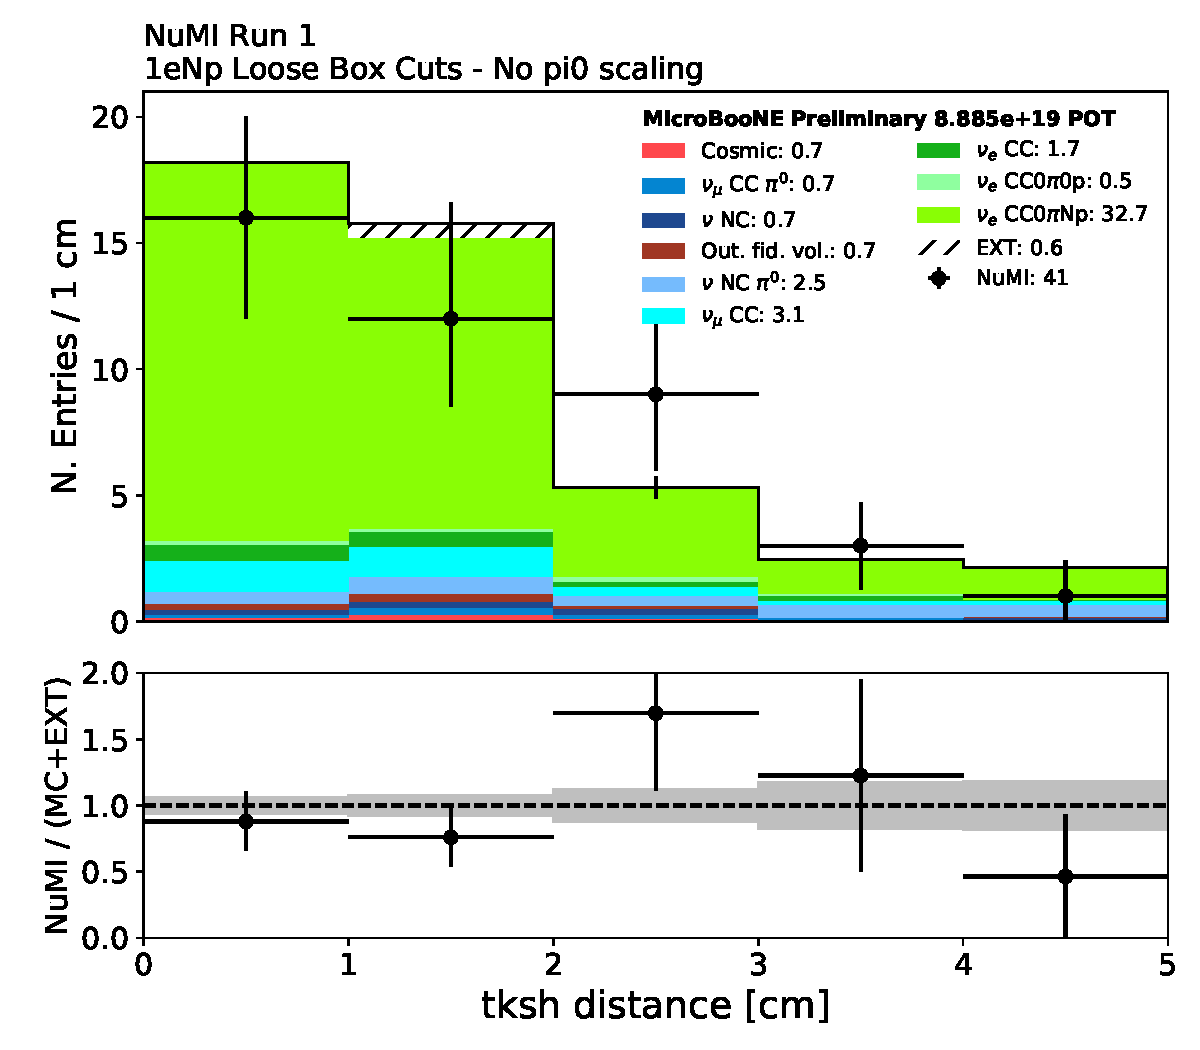
\includegraphics[width=1.0\textwidth]{Sidebands/Figures/NuMI/1eNp/tksh_distance.pdf}
    \caption{tksh\_distance}
    \end{subfigure}
    \begin{subfigure}{0.3\textwidth}
    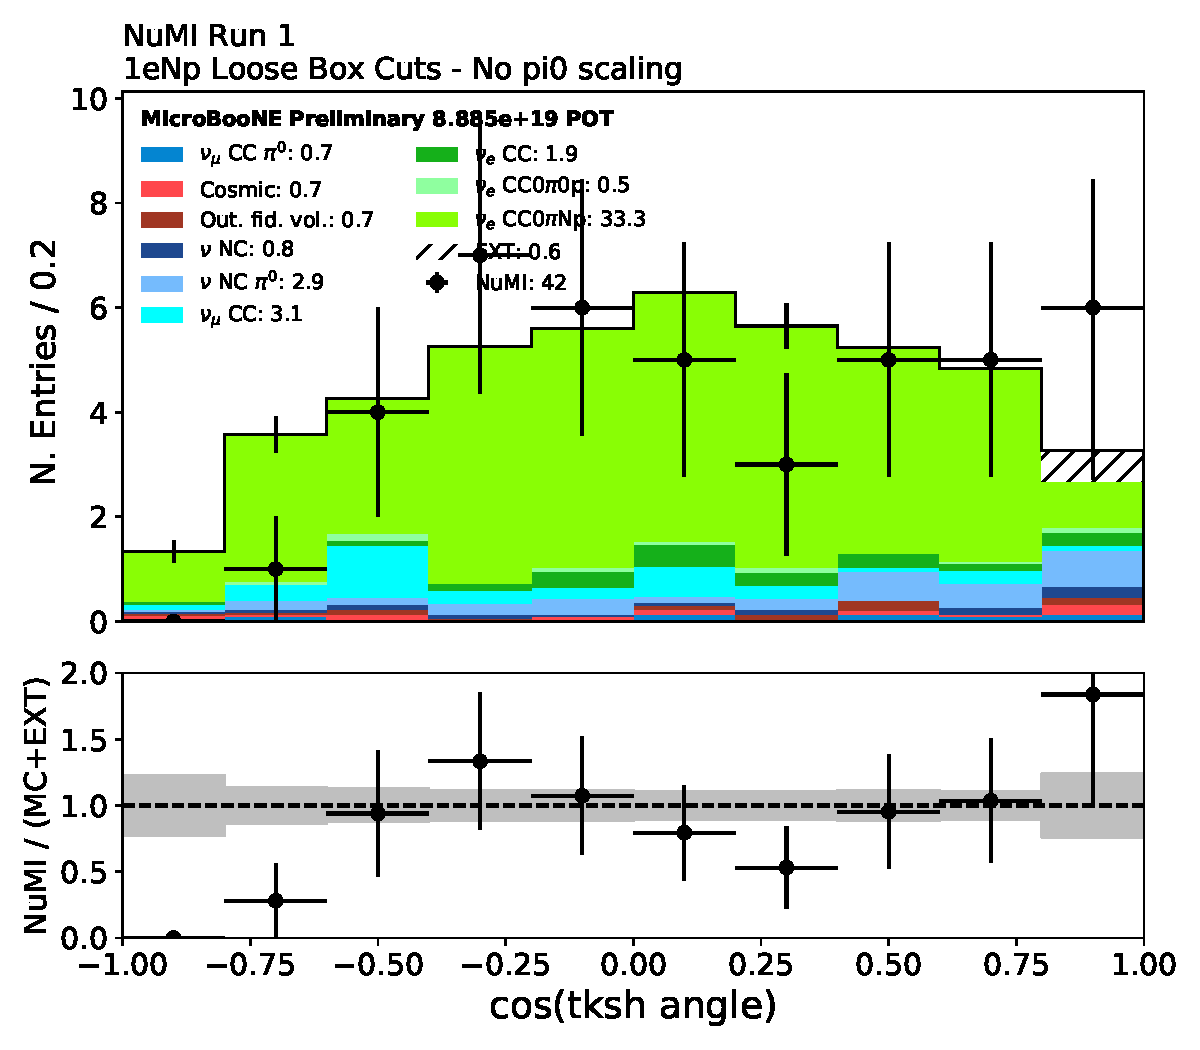
\includegraphics[width=1.0\textwidth]{Sidebands/Figures/NuMI/1eNp/tksh_angle.pdf}
    \caption{tksh\_angle}
    \end{subfigure}
    \begin{subfigure}{0.3\textwidth}
    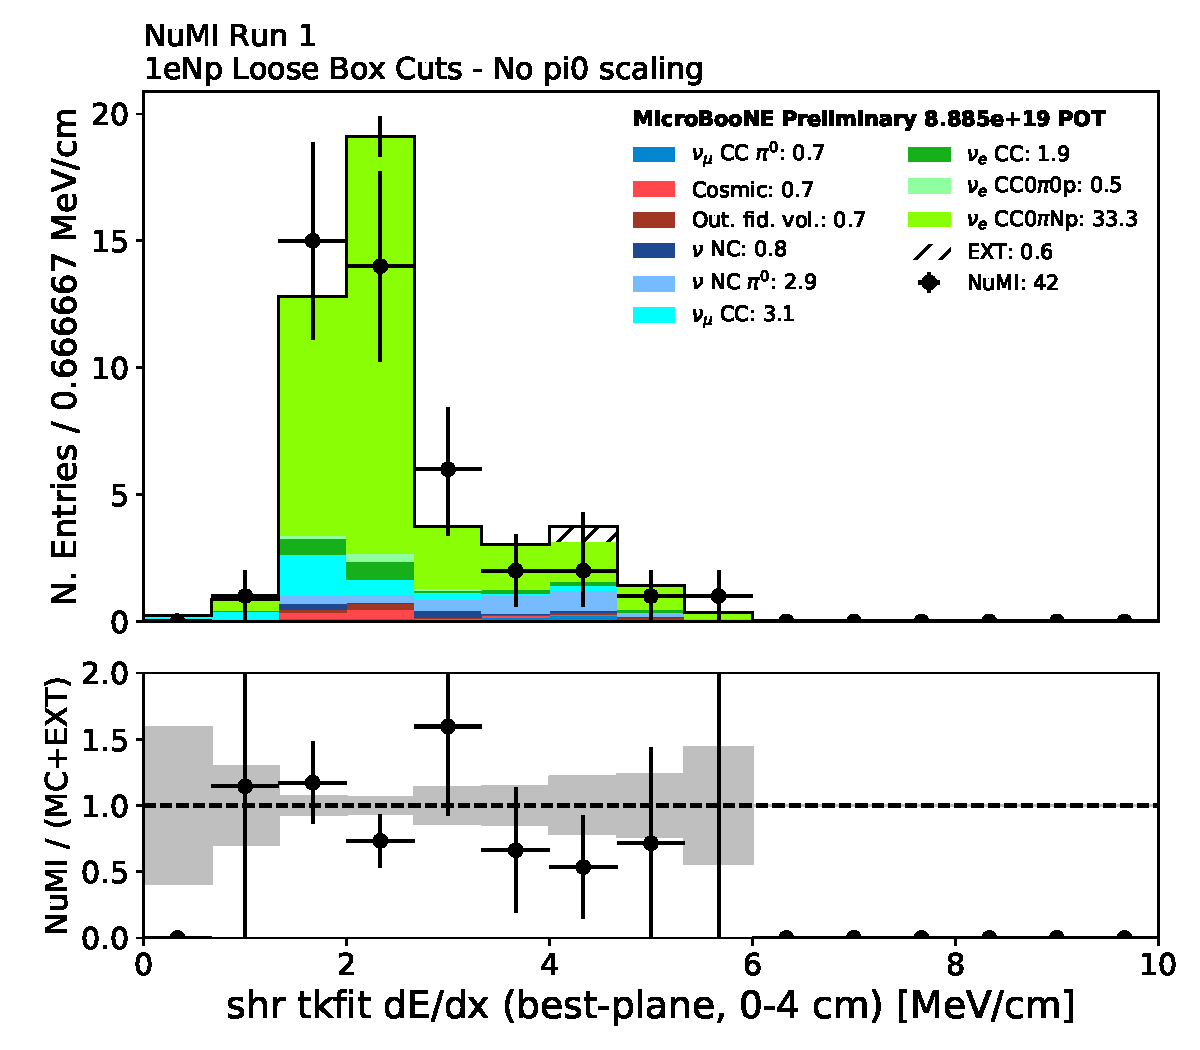
\includegraphics[width=1.0\textwidth]{Sidebands/Figures/NuMI/1eNp/shr_tkfit_dedx_max.pdf}
    \caption{shr\_tkfit\_dedx\_max}
    \end{subfigure}
    \caption{} 
    \label{fig:NuMI_1eNp_1}
\end{figure}

\begin{figure}[H]
    \centering
    \begin{subfigure}{0.3\textwidth}
    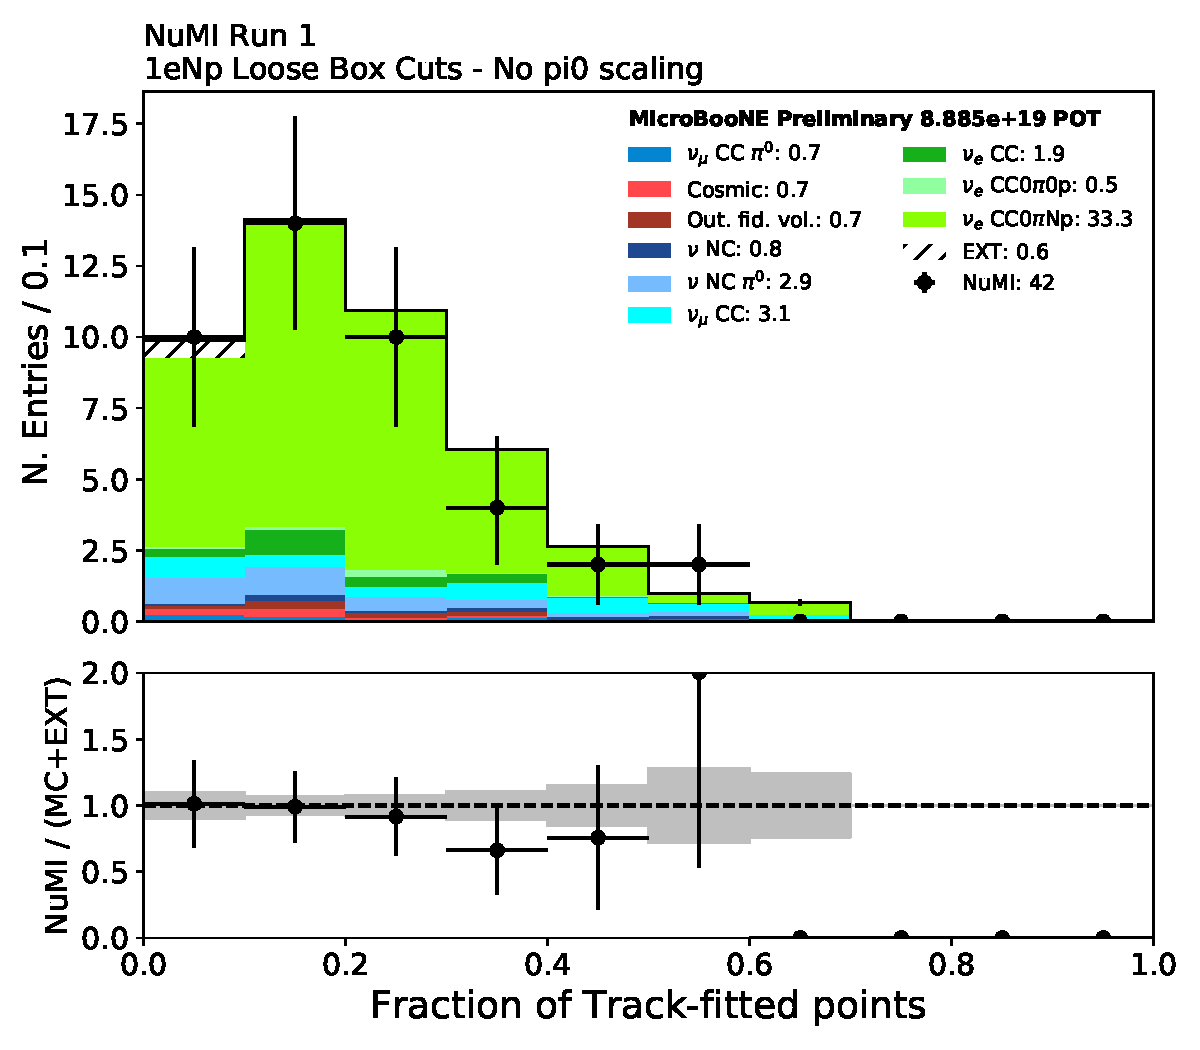
\includegraphics[width=1.0\textwidth]{Sidebands/Figures/NuMI/1eNp/trkfit.pdf}
    \caption{trkfit}
    \end{subfigure}
    \begin{subfigure}{0.3\textwidth}
    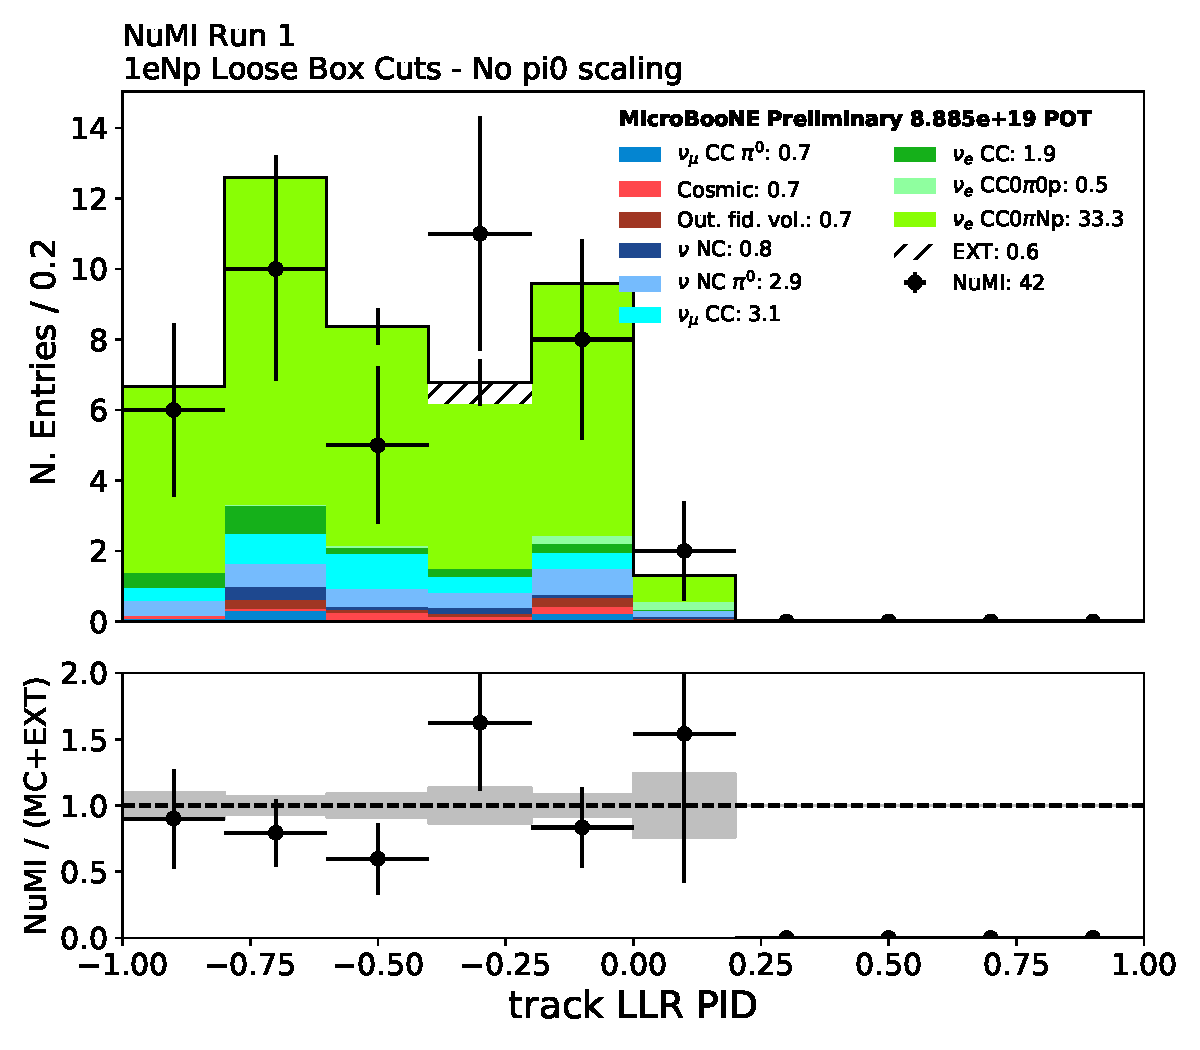
\includegraphics[width=1.0\textwidth]{Sidebands/Figures/NuMI/1eNp/trkpid.pdf}
    \caption{trkpid}
    \end{subfigure}
    \begin{subfigure}{0.3\textwidth}
    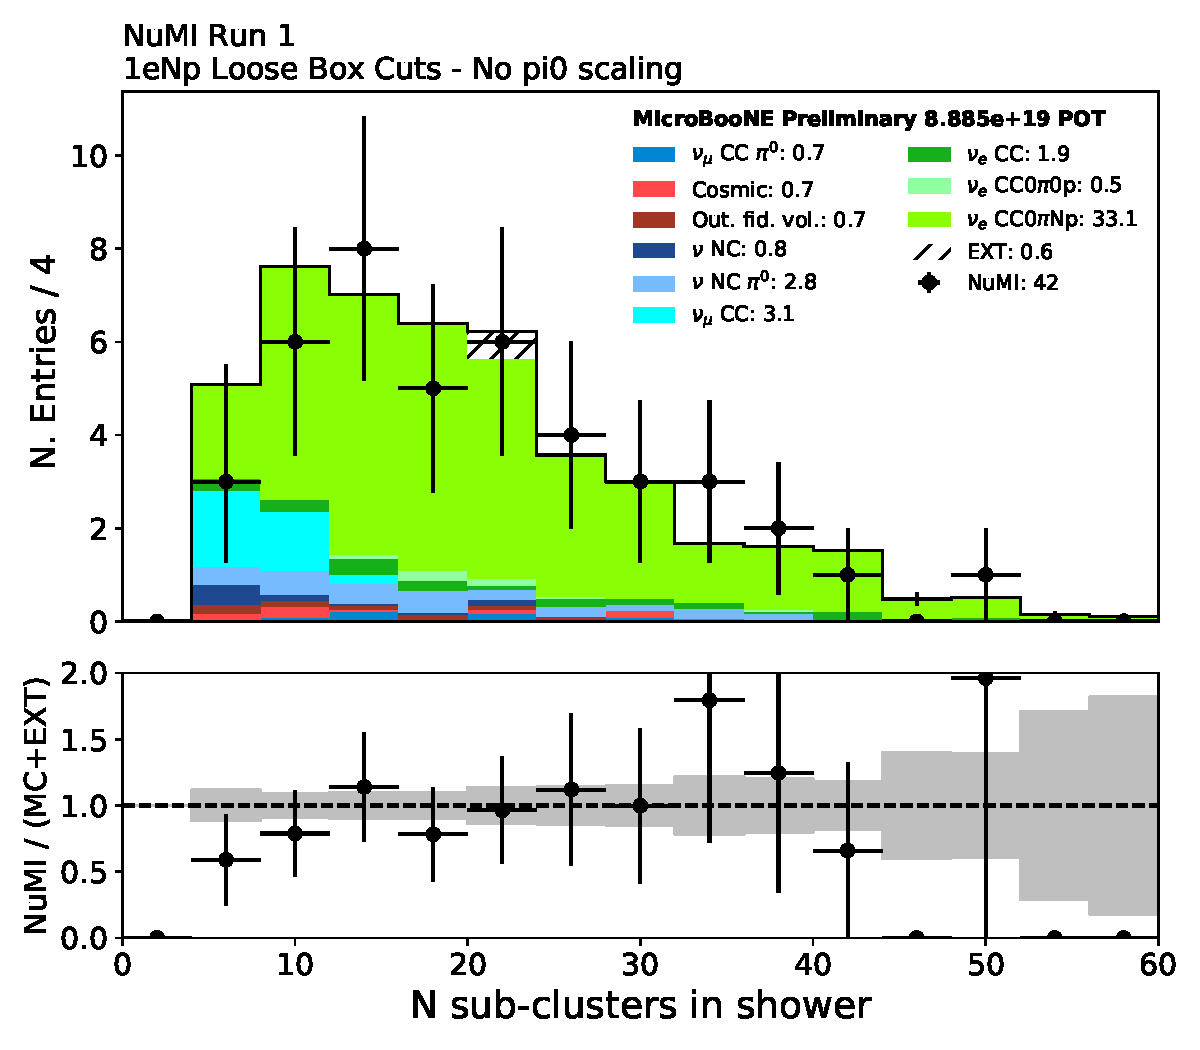
\includegraphics[width=1.0\textwidth]{Sidebands/Figures/NuMI/1eNp/subcluster.pdf}
    \caption{subcluster}
    \end{subfigure}
    \caption{} 
    \label{fig:NuMI_1eNp_2}
\end{figure}

\begin{figure}[H]
    \centering
    \begin{subfigure}{0.3\textwidth}
    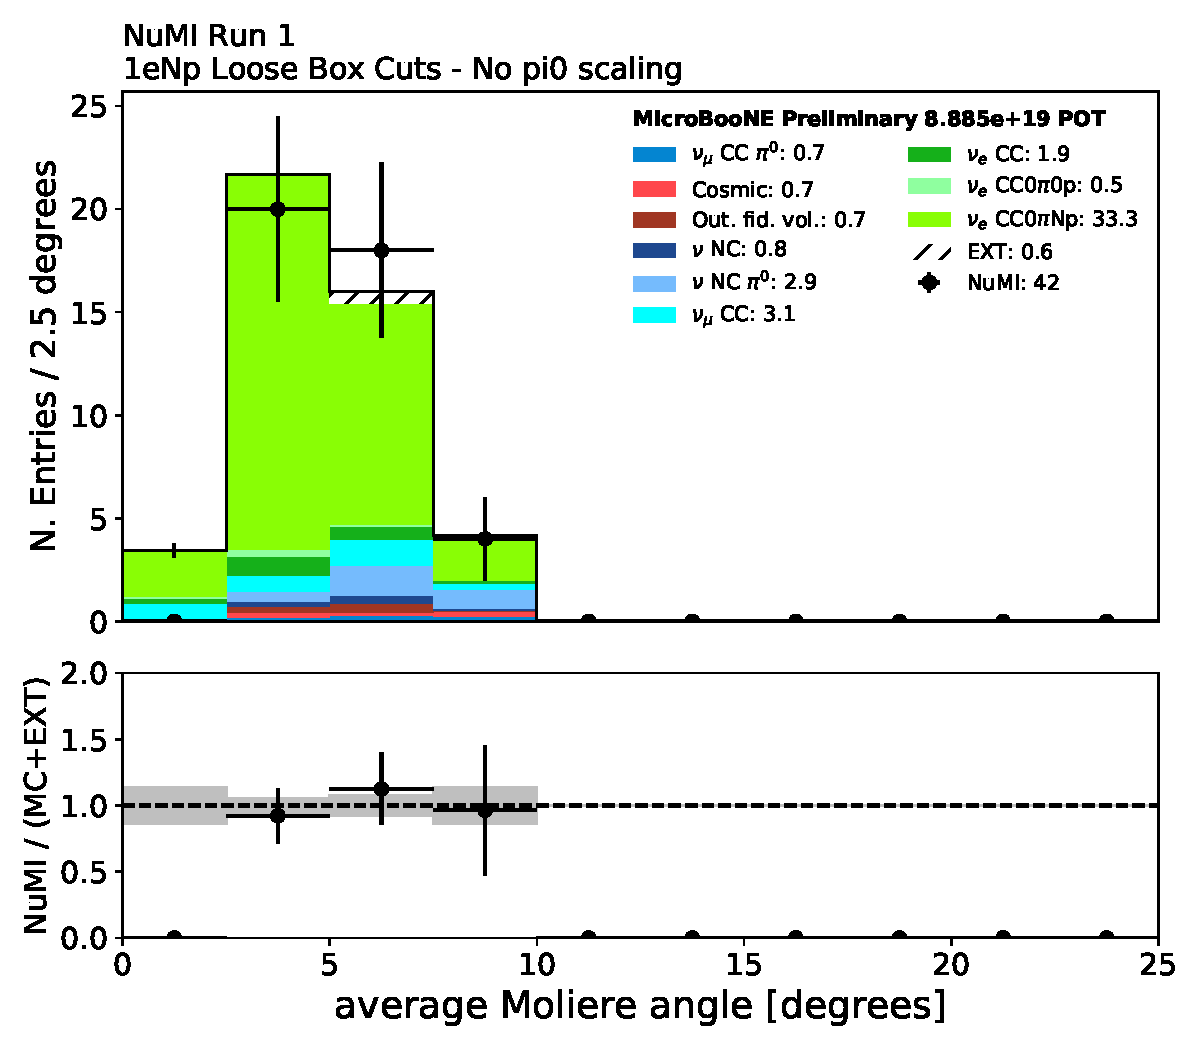
\includegraphics[width=1.0\textwidth]{Sidebands/Figures/NuMI/1eNp/shrmoliereavg.pdf}
    \caption{shrmoliereavg}
    \end{subfigure}
    \begin{subfigure}{0.3\textwidth}
    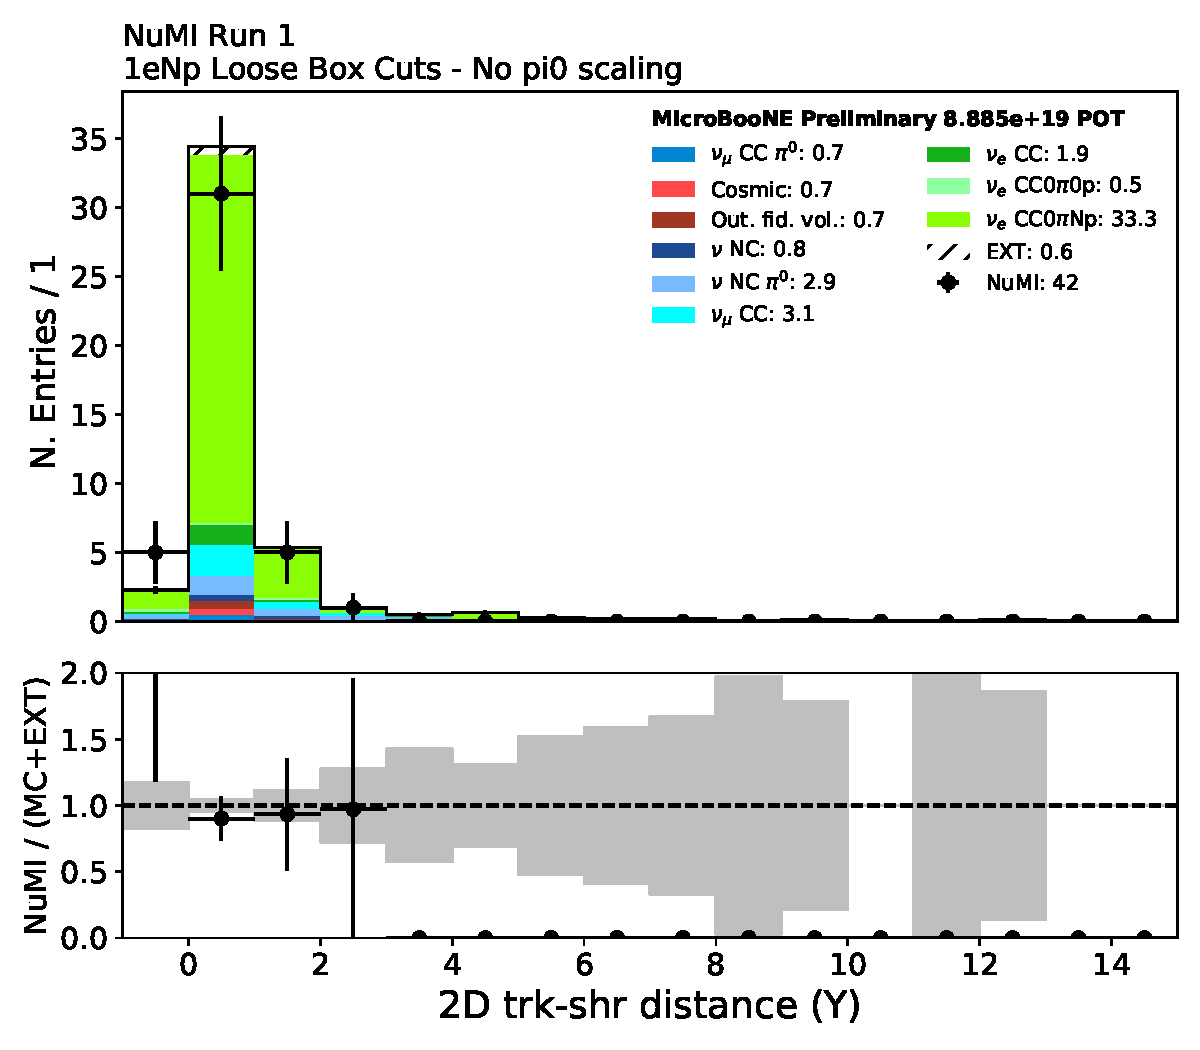
\includegraphics[width=1.0\textwidth]{Sidebands/Figures/NuMI/1eNp/trkshrhitdist2.pdf}
    \caption{tkshrhitdist2}
    \end{subfigure}
    \begin{subfigure}{0.3\textwidth}
    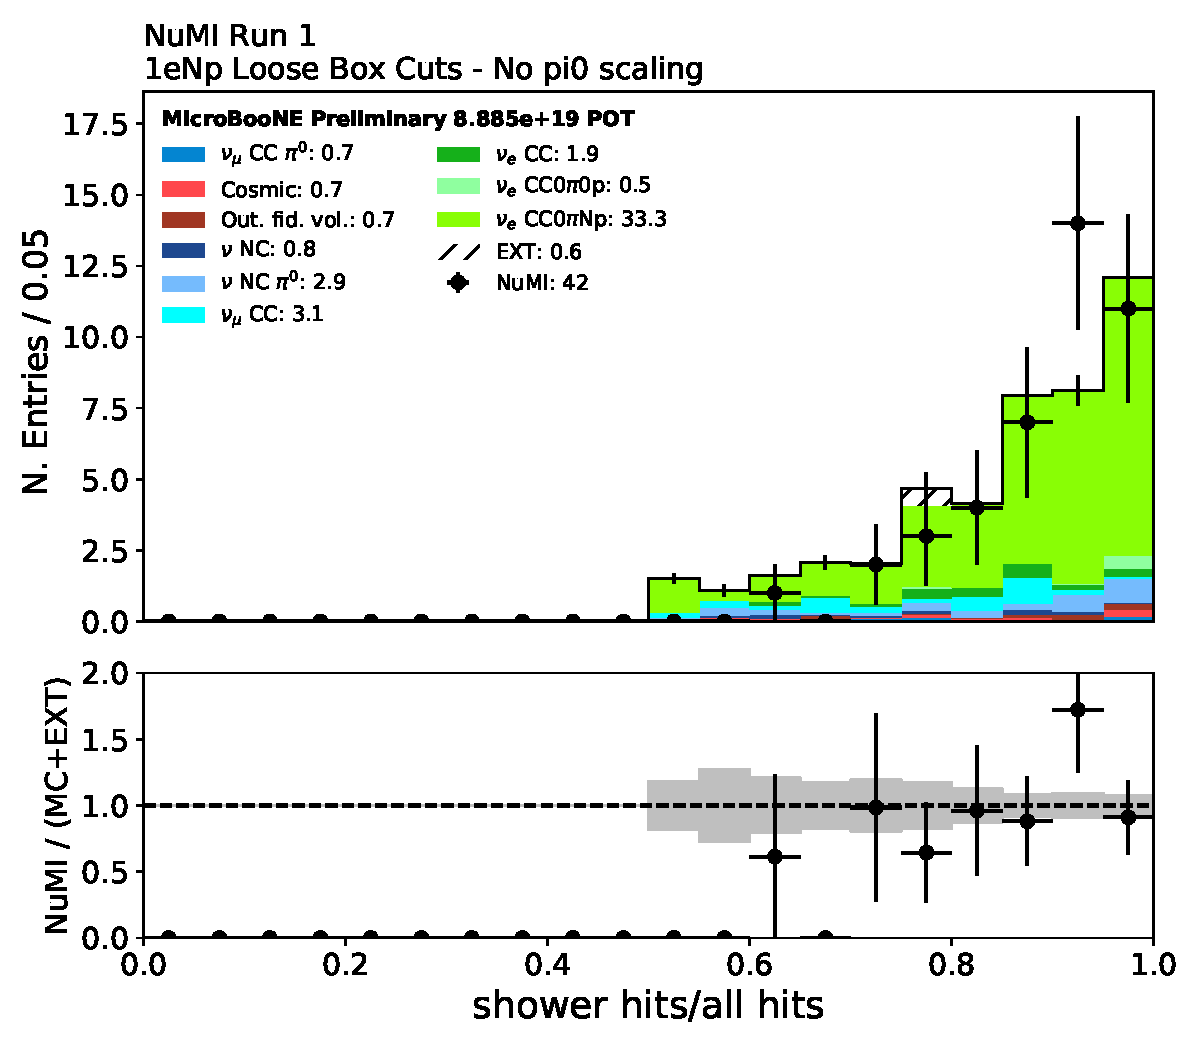
\includegraphics[width=1.0\textwidth]{Sidebands/Figures/NuMI/1eNp/hits_ratio.pdf}
    \caption{hits\_ratio}
    \end{subfigure}
    \caption{} 
    \label{fig:NuMI_1eNp_3}
\end{figure}

\begin{figure}[H]
    \centering
    \begin{subfigure}{0.3\textwidth}
    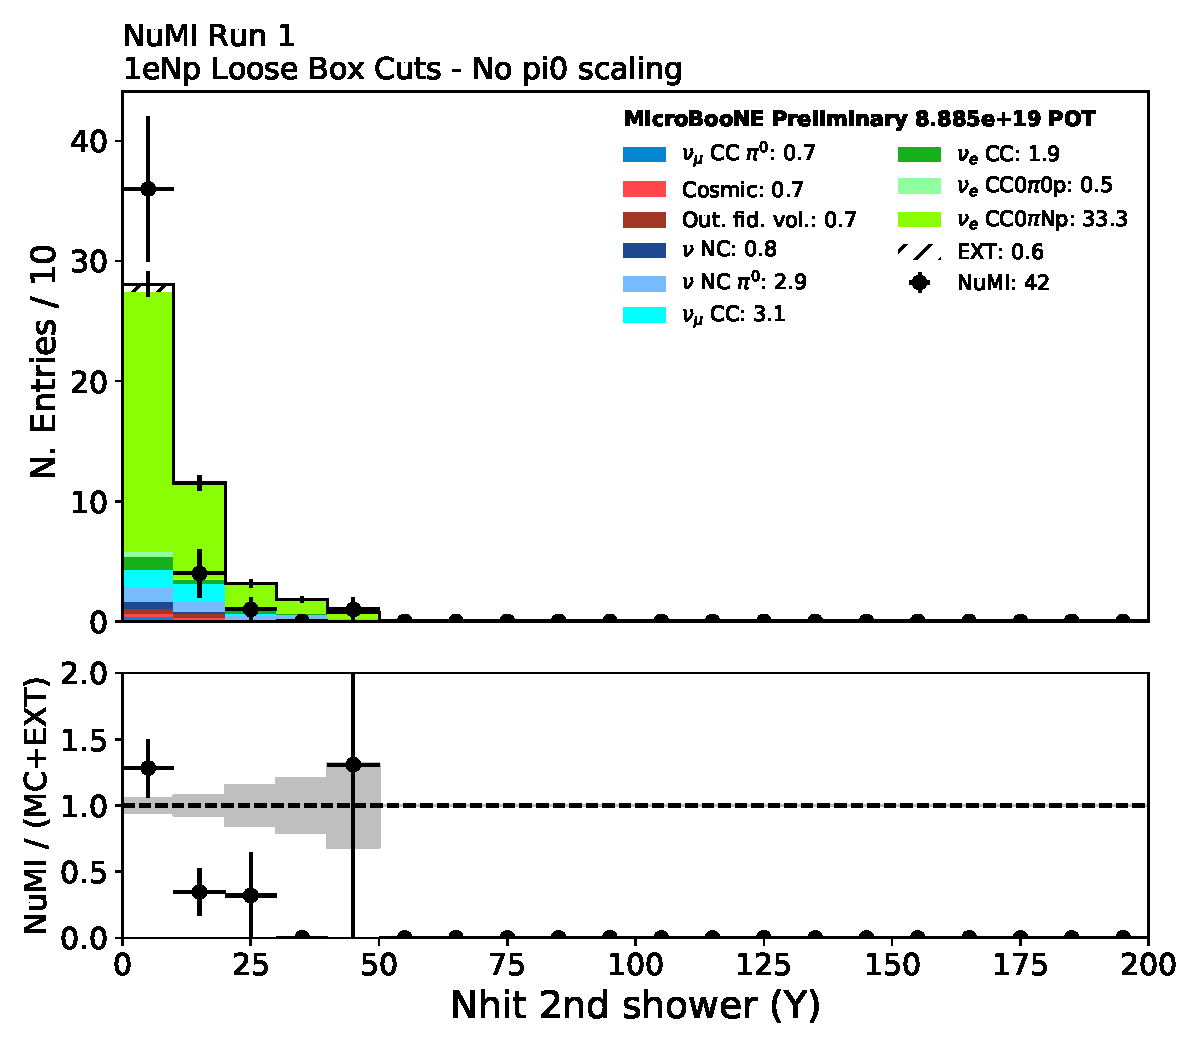
\includegraphics[width=1.0\textwidth]{Sidebands/Figures/NuMI/1eNp/secondshower_Y_nhit.pdf}
    \caption{secondshower\_Y\_nhit}
    \end{subfigure}
    \begin{subfigure}{0.3\textwidth}
    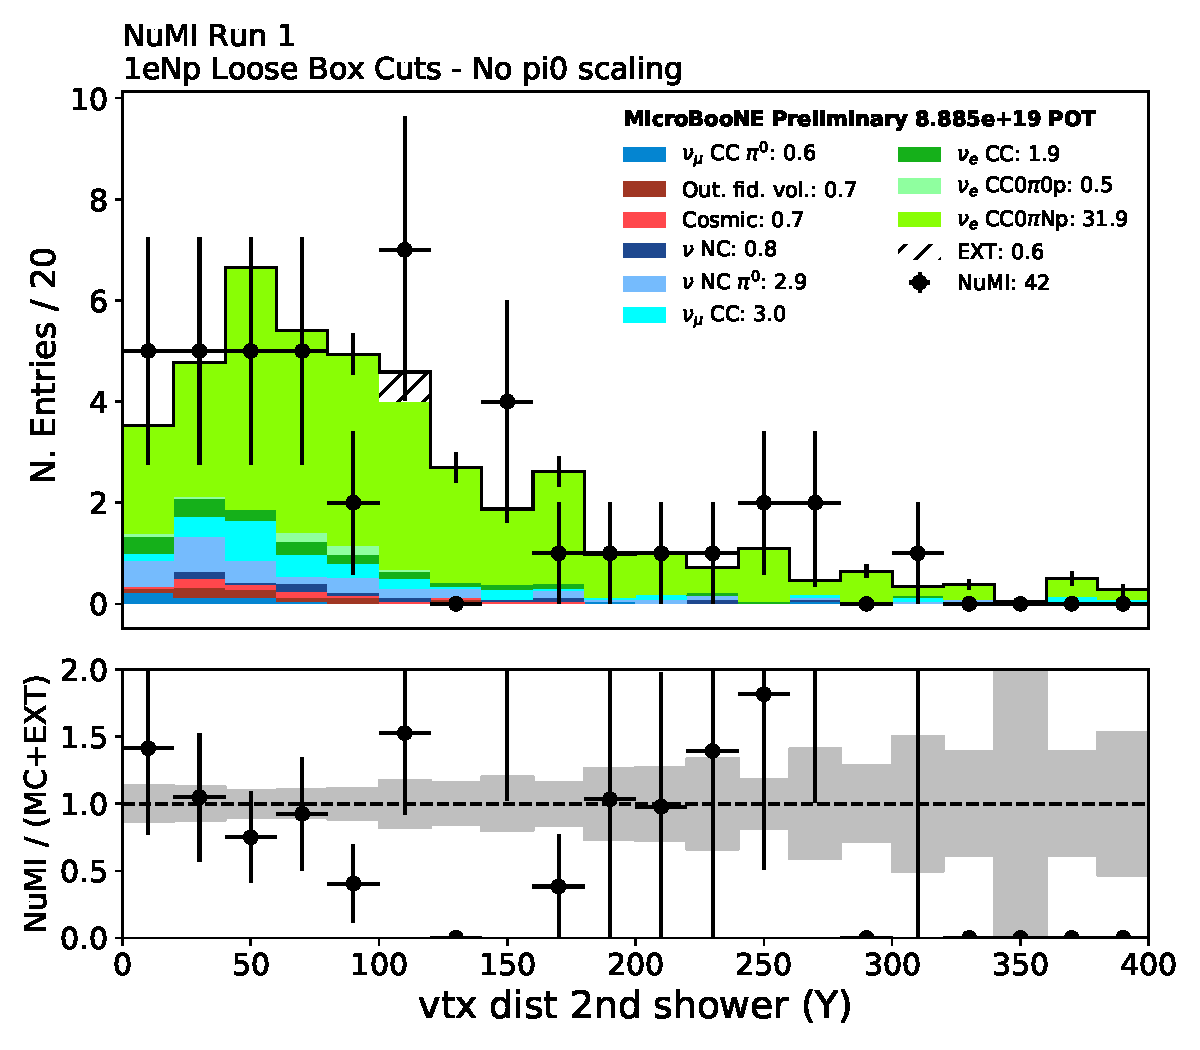
\includegraphics[width=1.0\textwidth]{Sidebands/Figures/NuMI/1eNp/secondshower_Y_vtxdist.pdf}
    \caption{secondshower\_Y\_vtxdist}
    \end{subfigure}
    \begin{subfigure}{0.3\textwidth}
    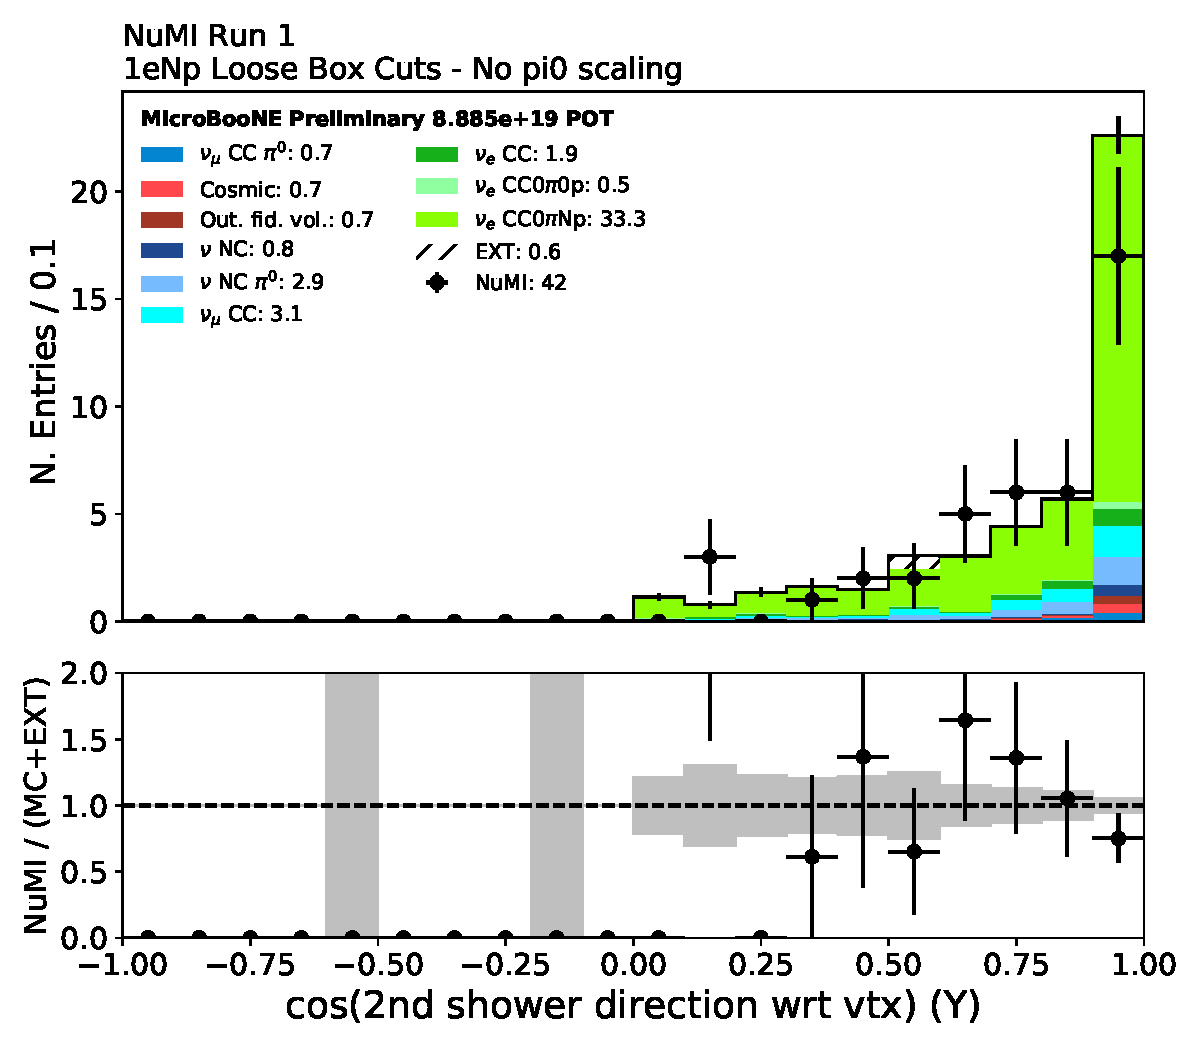
\includegraphics[width=1.0\textwidth]{Sidebands/Figures/NuMI/1eNp/secondshower_Y_dot.pdf}
    \caption{secondshower\_Y\_dot}
    \end{subfigure}
    \caption{} 
    \label{fig:NuMI_1eNp_4}
\end{figure}

\begin{figure}[H]
    \centering
    \begin{subfigure}{0.3\textwidth}
    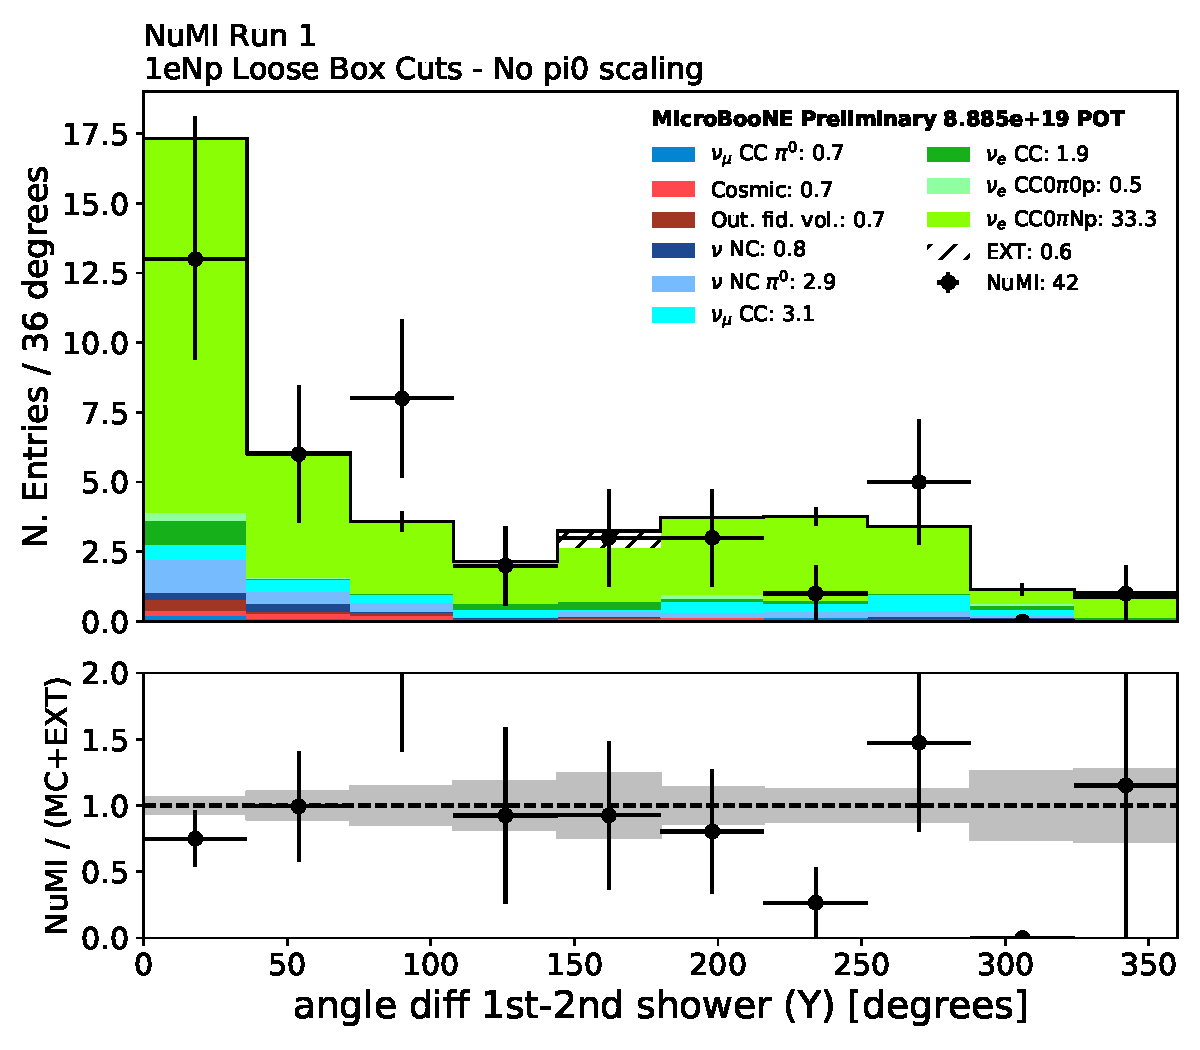
\includegraphics[width=1.0\textwidth]{Sidebands/Figures/NuMI/1eNp/anglediff_Y.pdf}
    \caption{anglediff\_Y}
    \end{subfigure}
    \begin{subfigure}{0.3\textwidth}
    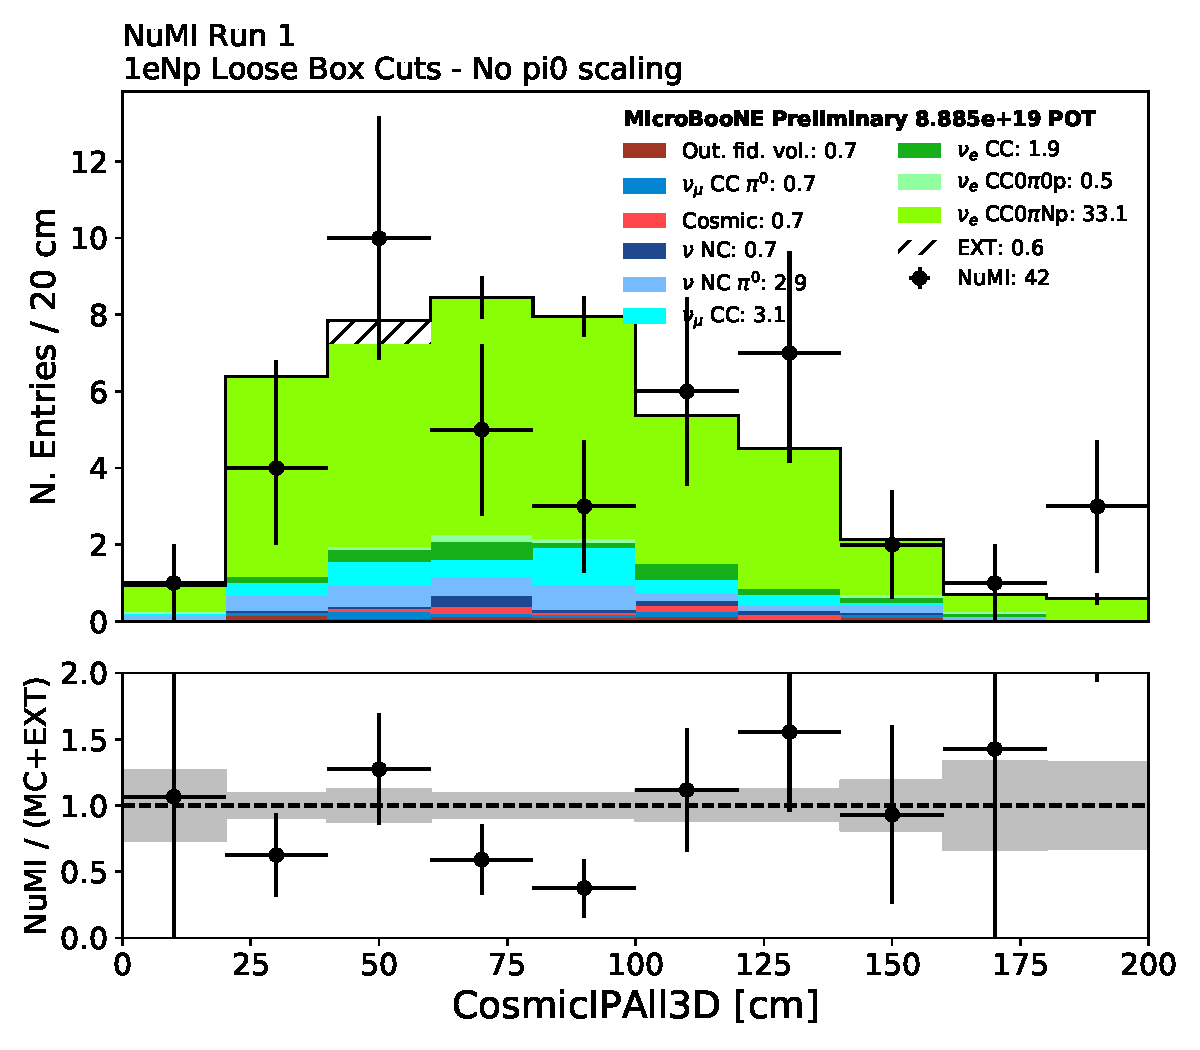
\includegraphics[width=1.0\textwidth]{Sidebands/Figures/NuMI/1eNp/CosmicIPAll3D.pdf}
    \caption{CosmicIPAll3D}
    \end{subfigure}
    \begin{subfigure}{0.3\textwidth}
    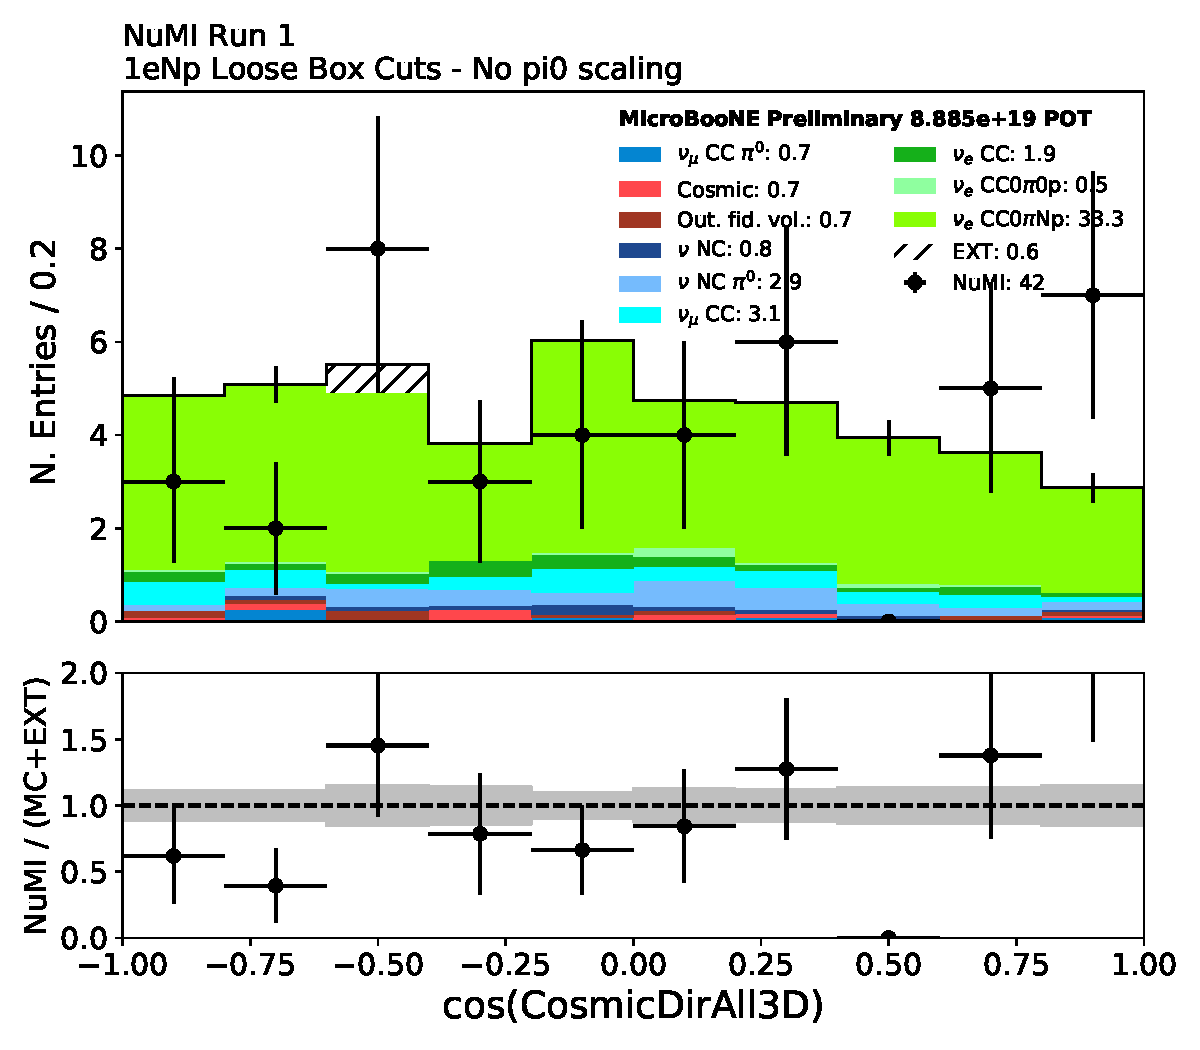
\includegraphics[width=1.0\textwidth]{Sidebands/Figures/NuMI/1eNp/CosmicDirAll3D.pdf}
    \caption{CosmidDirAll3D}
    \end{subfigure}
    \caption{} 
    \label{fig:NuMI_1eNp_5}
\end{figure}


Figures~\ref{fig:NuMI_1eNp_7} show the BDT response from the \npsel NuMI sideband.

\begin{figure}[H]
    \centering
    \begin{subfigure}{0.4\textwidth}
    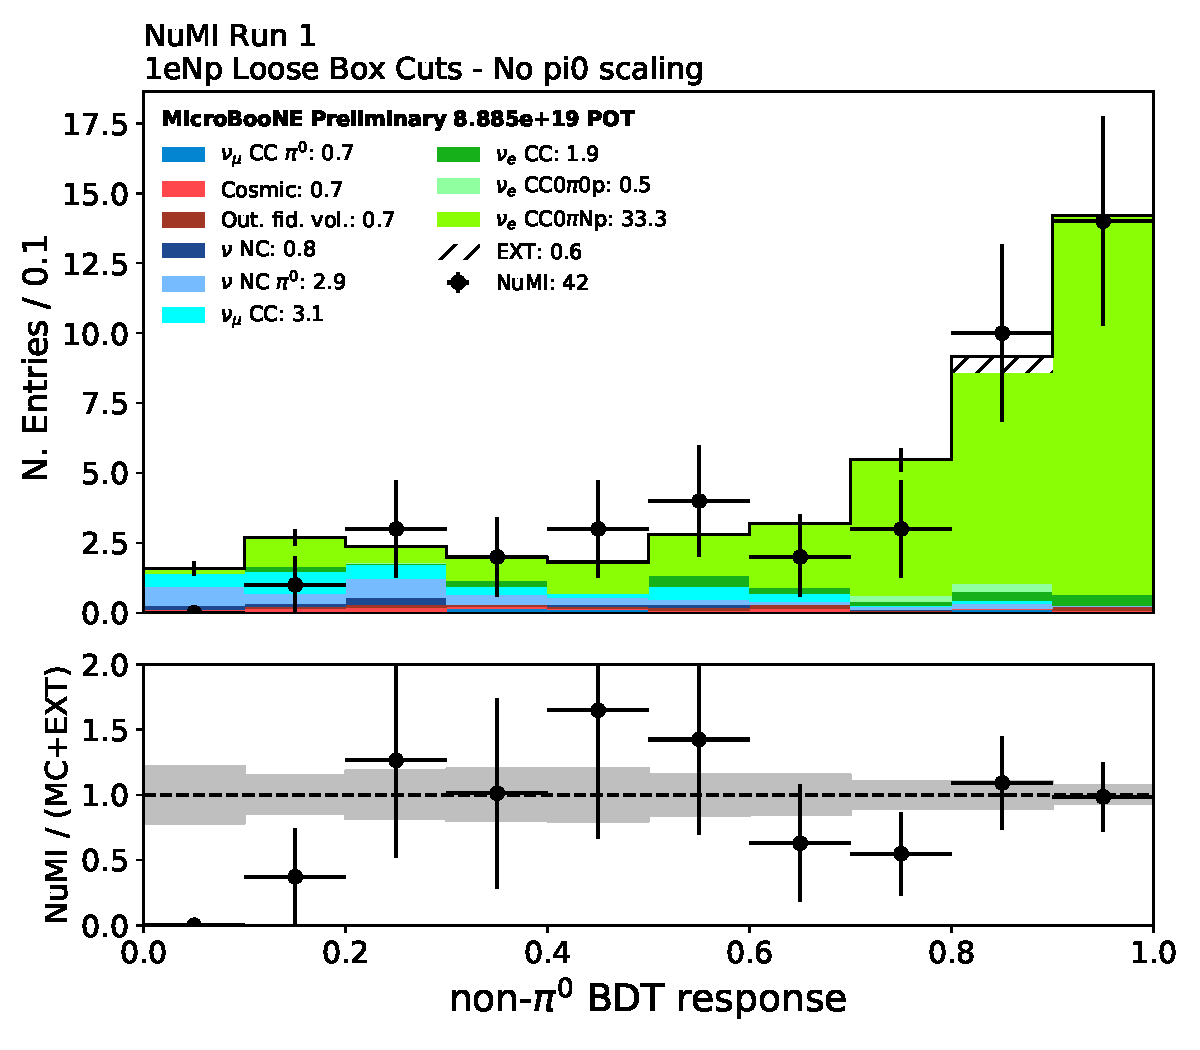
\includegraphics[width=1.0\textwidth]{Sidebands/Figures/NuMI/1eNp/nonpi0_score.pdf}
    \caption{Non $\pi^0$ BDT}
    \end{subfigure}
    \begin{subfigure}{0.4\textwidth}
    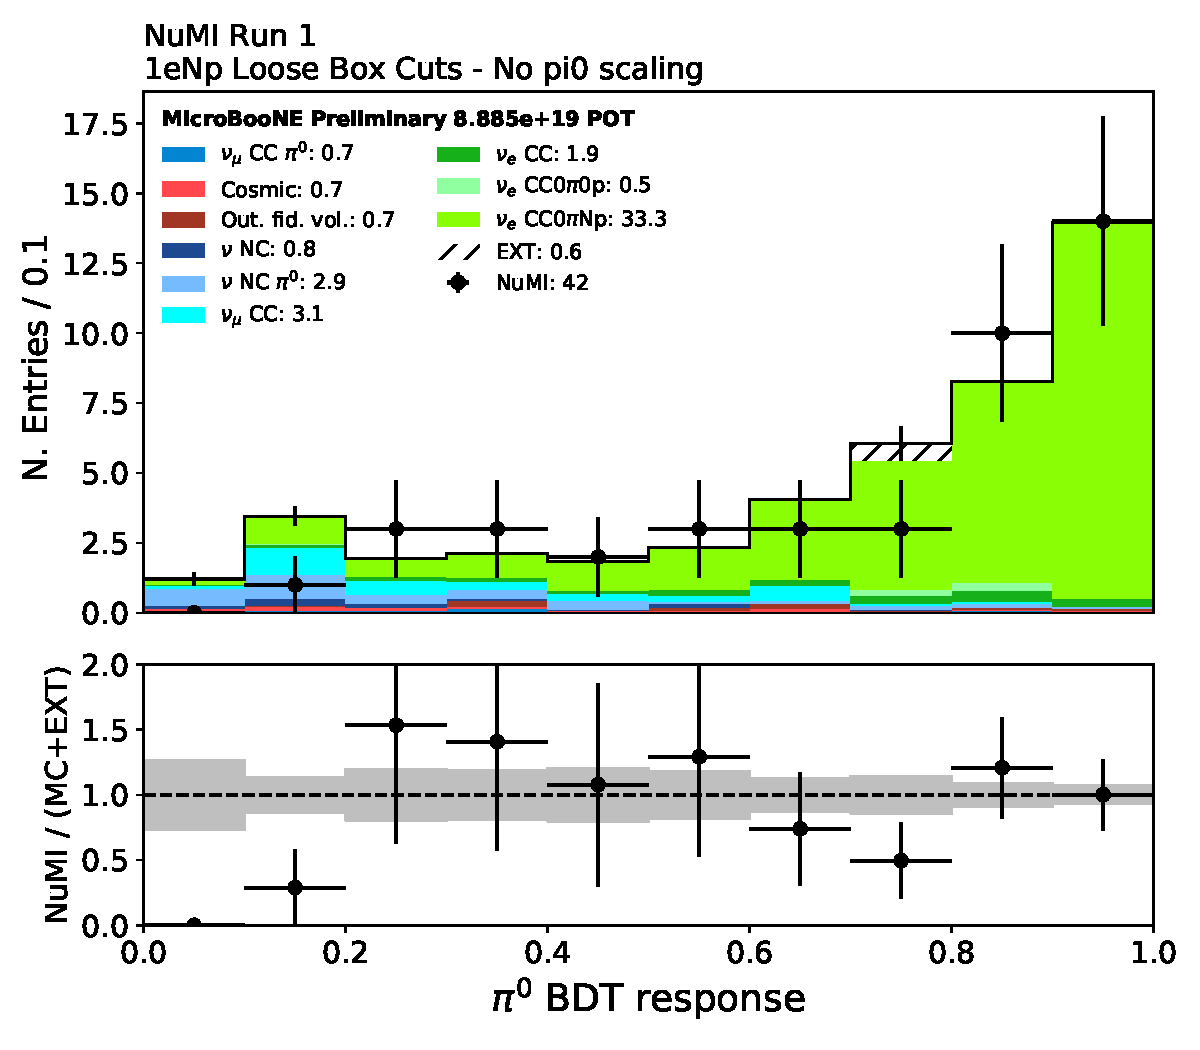
\includegraphics[width=1.0\textwidth]{Sidebands/Figures/NuMI/1eNp/pi0_score.pdf}
    \caption{$\pi^0$ BDT}
    \end{subfigure}
    \caption{} 
    \label{fig:NuMI_1eNp_7}
\end{figure}


\begin{comment}
\begin{table}[H]
\centering
\setlength{\tabcolsep}{10pt}
\renewcommand{\arraystretch}{1.25}
\begin{tabular}{| c | c | c | c | c | c | c | } 
 \hline
\multirow{3}{*}{variable} & \multicolumn{6}{c|}{p-values} \\
\cline{2-7} & \multicolumn{3}{c|}{pre-selection} & \multicolumn{3}{c|}{loose cuts}  \\ 
\cline{2-7} & stat-only & diag syst. & covariance & stat-only & diag syst. & covariance \\ \hline
n\_showers\_contained & 0.524 & 0.944 & 0.944 & 0.401 & 0.614 & 0.614 \\ \hline
n\_tracks\_contained & 0.046 & 0.989 & 0.229 & 0.038 & 0.105 & 0.074 \\ \hline
reco\_e & 0.265 & 0.989 & 0.606 & 0.337 & 0.516 & 0.475 \\ \hline
hits\_ratio & 0.066 & 0.995 & 0.222 & 0.021 & 0.094 & 0.070 \\ \hline
CosmicIPAll3D & 0.469 & 0.999 & 0.668 & 0.152 & 0.287 & 0.299 \\ \hline
CosmicDirAll3D & 0.006 & 0.997 & 0.038 & 0.683 & 0.826 & 0.820 \\ \hline
trkfit & 0.023 & 0.929 & 0.332 & 0.396 & 0.567 & 0.560 \\ \hline
shrmoliereavg & 0.653 & 0.987 & 0.827 & 0.888 & 0.949 & 0.969 \\ \hline
shr\_score & 0.364 & 0.998 & 0.787 & 0.044 & 0.084 & 0.078 \\ \hline
subcluster & 0.003 & 0.419 & 0.021 & 0.274 & 0.483 & 0.433 \\ \hline
secondshower\_Y\_nhit & 0.026 & 0.761 & 0.141 & 0.248 & 0.369 & 0.358 \\ \hline
secondshower\_Y\_dot & 0.825 & 0.998 & 0.946 & 0.928 & 0.972 & 0.975 \\ \hline
anglediff\_Y & 0.034 & 0.996 & 0.190 & 0.340 & 0.539 & 0.555 \\ \hline
secondshower\_Y\_vtxdist & 0.746 & 1.000 & 0.886 & 0.740 & 0.871 & 0.845 \\ \hline
shr\_tkfit\_dedx\_max & 0.021 & 0.982 & 0.189 & 0.454 & 0.574 & 0.555 \\ \hline
shr\_trk\_sce\_start\_y & 0.097 & 0.996 & 0.217 & 0.458 & 0.667 & 0.658 \\ \hline
shr\_trk\_sce\_end\_y & 0.071 & 0.999 & 0.244 & 0.083 & 0.215 & 0.207 \\ \hline
tksh\_angle & 0.385 & 1.000 & 0.669 & 0.996 & 0.999 & 0.999 \\ \hline
trkshrhitdist2 & 0.131 & 0.989 & 0.297 & 0.945 & 0.978 & 0.979 \\ \hline
tksh\_distance & 0.081 & 0.980 & 0.293 & 0.424 & 0.623 & 0.571 \\ \hline
trkpid & 0.000 & 0.006 & 0.000 & 0.854 & 0.920 & 0.912 \\ \hline
nonpi0\_score & 0.006 & 0.129 & 0.037 & 0.000 & 0.006 & 0.003 \\ \hline
pi0\_score & 0.193 & 0.694 & 0.546 & 0.016 & 0.105 & 0.080 \\ \hline
 \end{tabular}
 \caption{\label{tab:HiENPpvalues}p-values from the high-energy \npsel sideband for input variables to the \npsel in addition to the final BDT scores (\texttt{pi0\_score}, \texttt{nonpi0\_score}) and the reconstructed energy spectrum \texttt{reco\_e}. The three columns show the p-values computed through statistics-only uncertainties (left), with systematics but not accounting for correlations in systematics (center), and finally including the full systematics covariance matrix. Systematics include flux, cross-sections, and re-interaction uncertainties, but not detector uncertainties.}
\end{table}
\end{comment}

Figures~\ref{fig:NuMI_1eNp_9} and~\ref{fig:NuMI_1eNp_10} show select kinematics distributions for selected \npsel events.

\begin{figure}[H]
    \centering
    \begin{subfigure}{0.3\textwidth}
    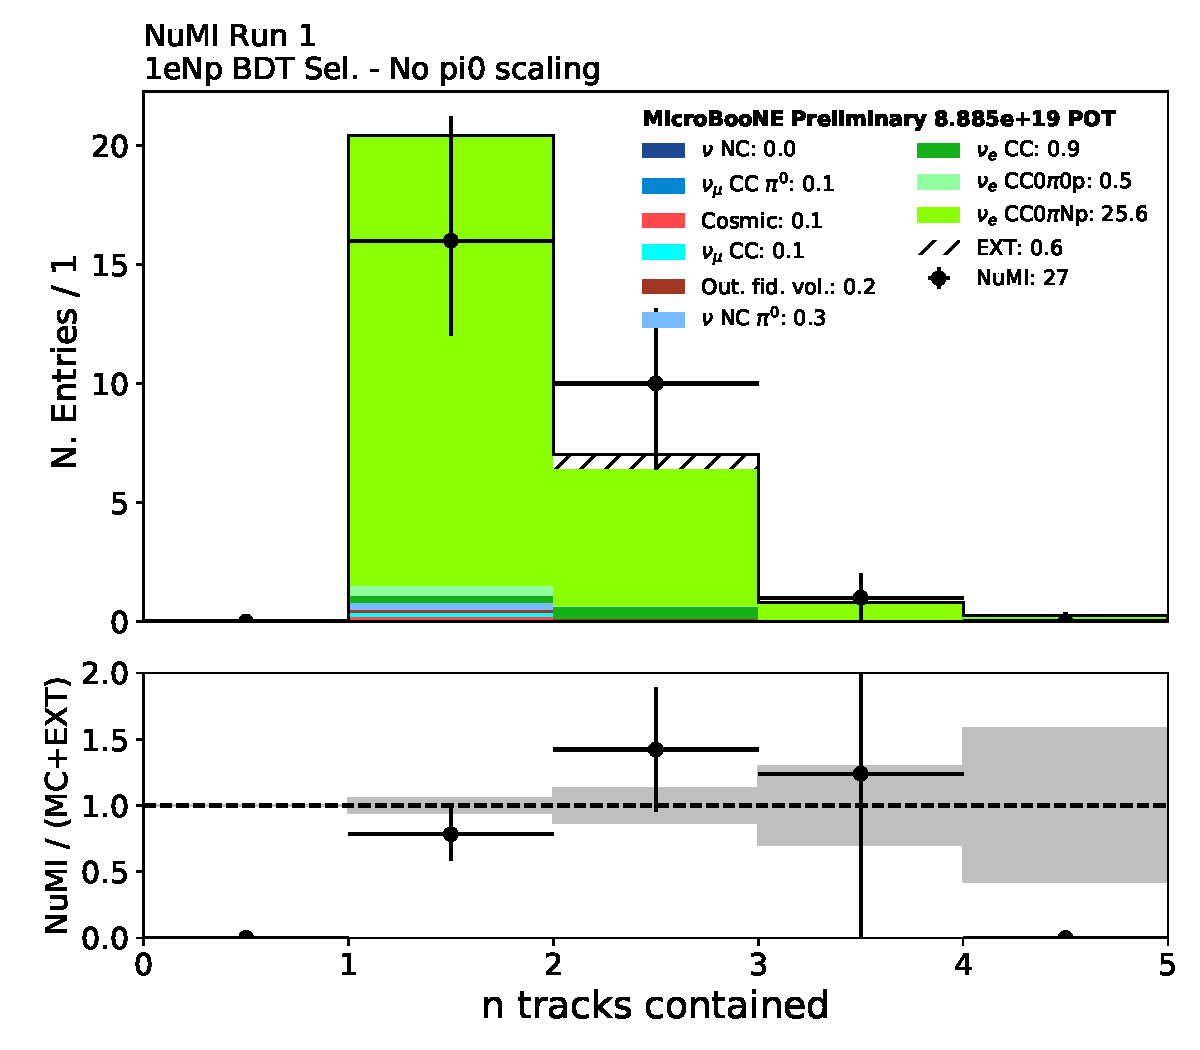
\includegraphics[width=1.0\textwidth]{Sidebands/Figures/NuMI/1eNp/BDTSel/n_tracks_contained.pdf}
    \caption{}
    \end{subfigure}
    \begin{subfigure}{0.3\textwidth}
    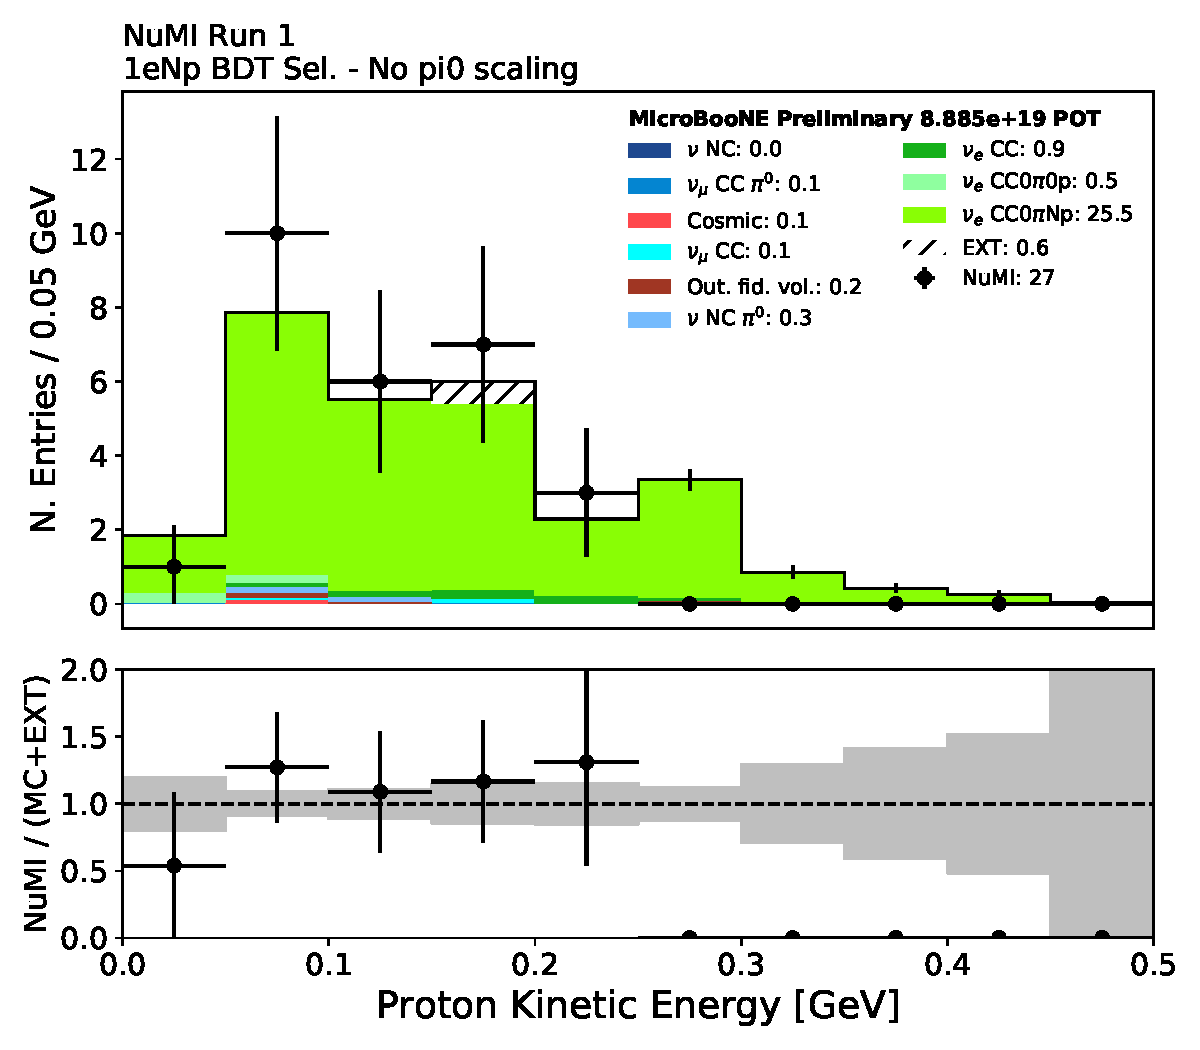
\includegraphics[width=1.0\textwidth]{Sidebands/Figures/NuMI/1eNp/BDTSel/protonenergy.pdf}
    \caption{}
    \end{subfigure}
    \begin{subfigure}{0.3\textwidth}
    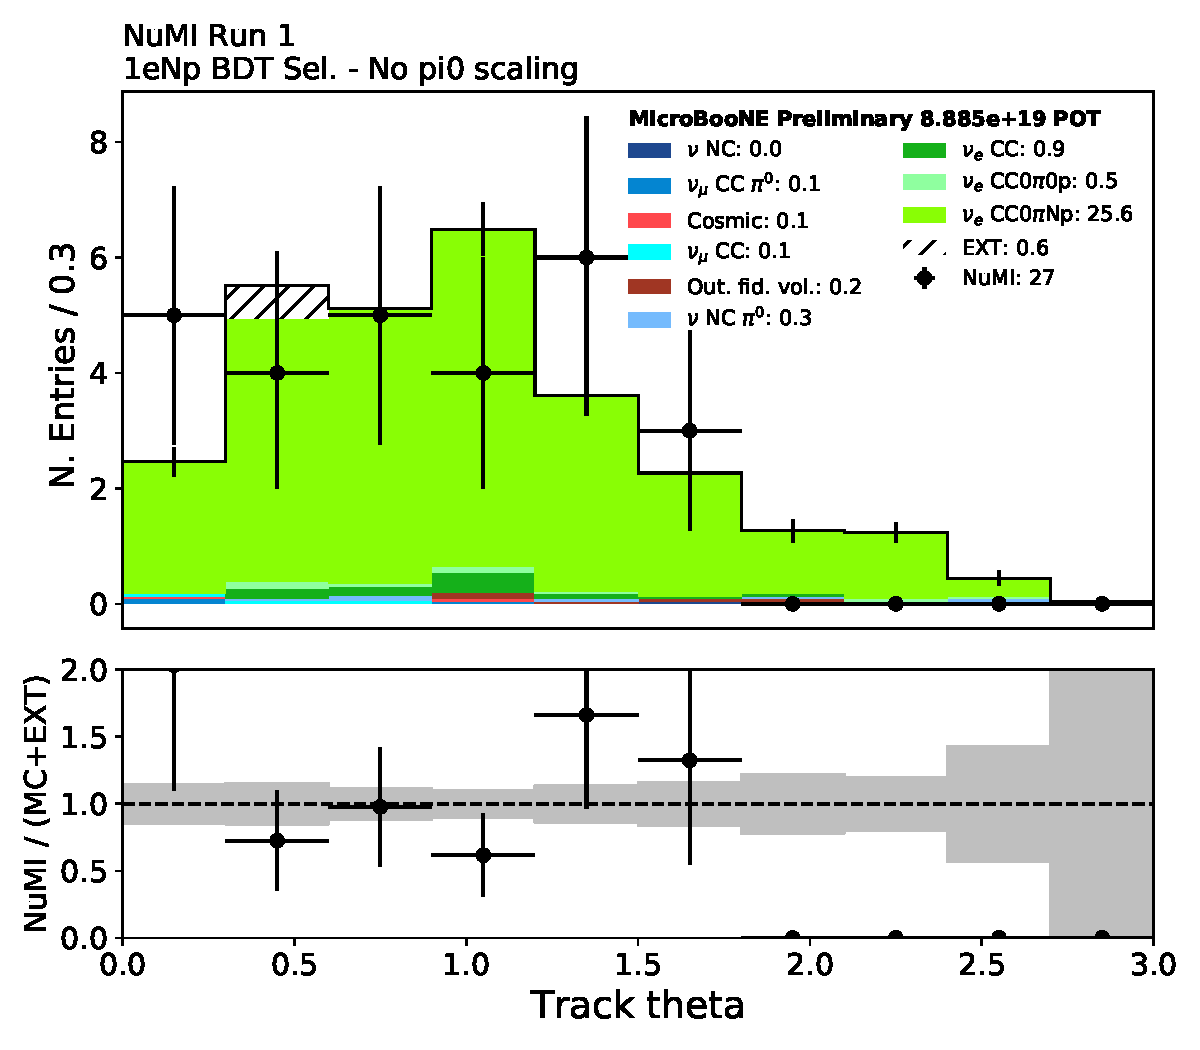
\includegraphics[width=1.0\textwidth]{Sidebands/Figures/NuMI/1eNp/BDTSel/trk_theta.pdf}
    \caption{}
    \end{subfigure}
    \caption{} 
    \label{fig:NuMI_1eNp_9}
\end{figure}

\begin{figure}[H]
    \centering
    \begin{subfigure}{0.3\textwidth}
    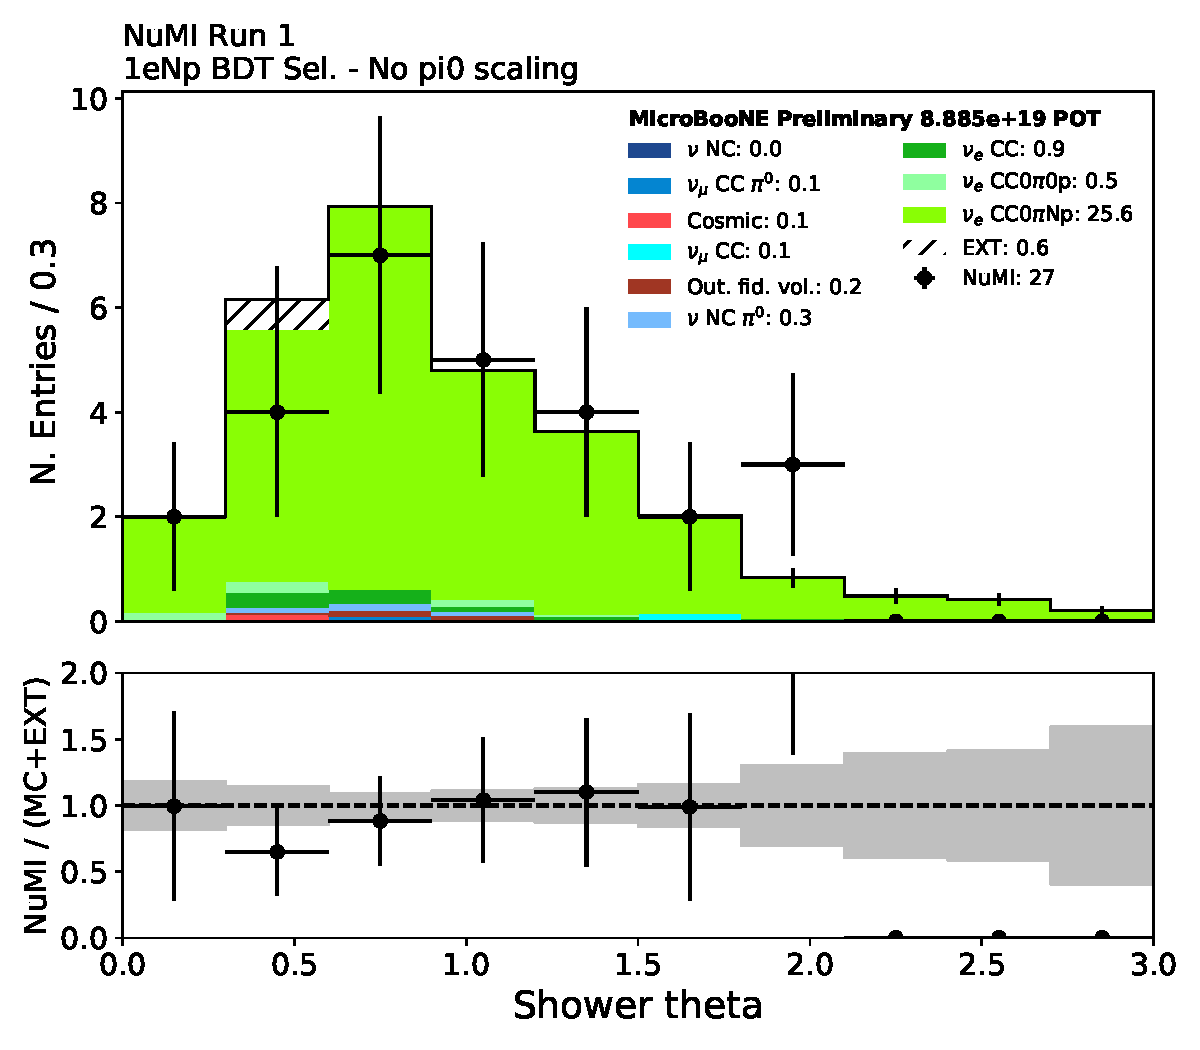
\includegraphics[width=1.0\textwidth]{Sidebands/Figures/NuMI/1eNp/BDTSel/shr_theta.pdf}
    \caption{}
    \end{subfigure}
    \begin{subfigure}{0.3\textwidth}
    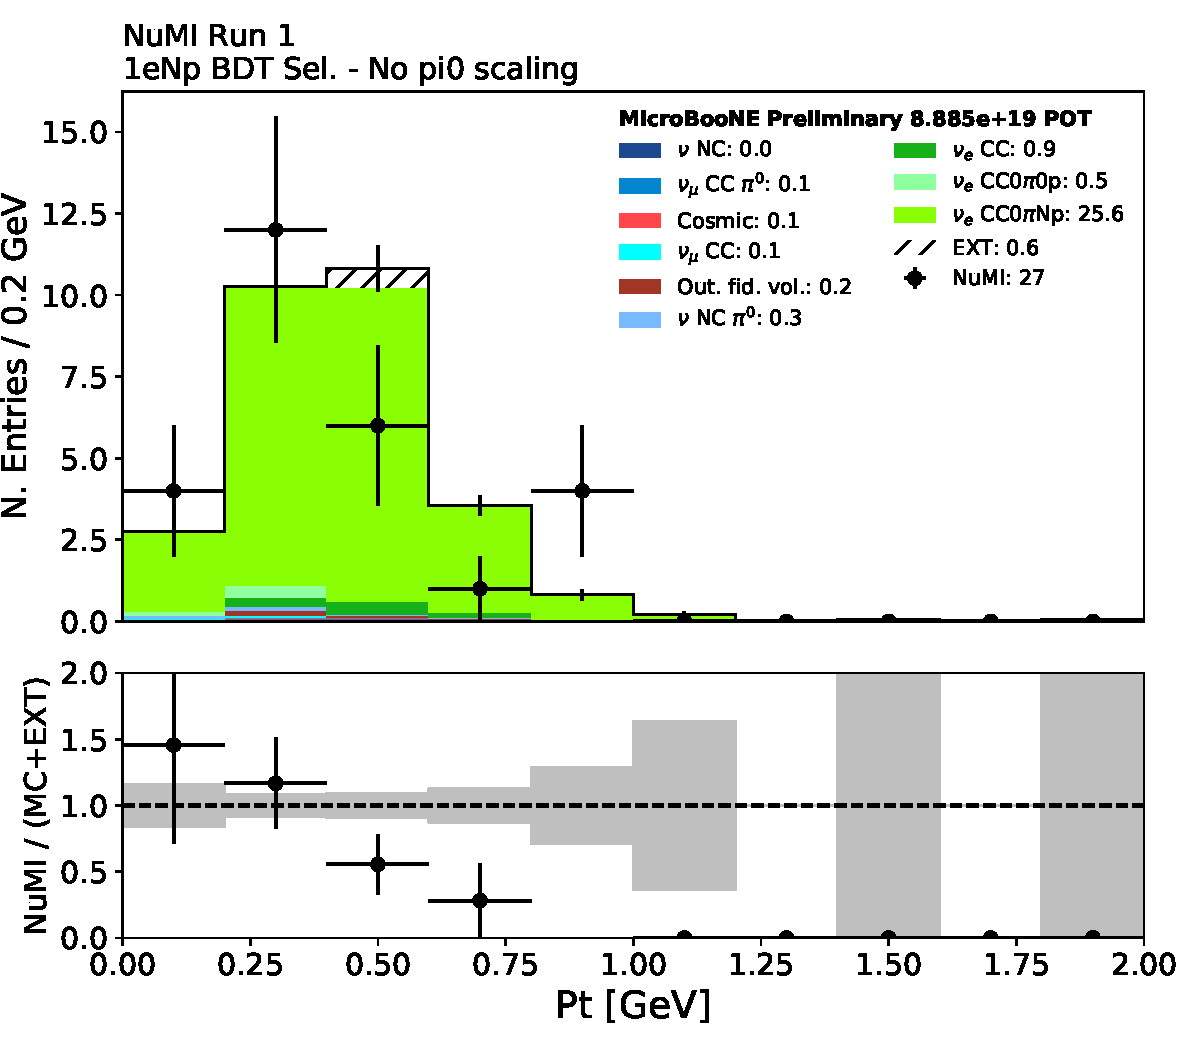
\includegraphics[width=1.0\textwidth]{Sidebands/Figures/NuMI/1eNp/BDTSel/pt.pdf}
    \caption{}
    \end{subfigure}
    \begin{subfigure}{0.3\textwidth}
    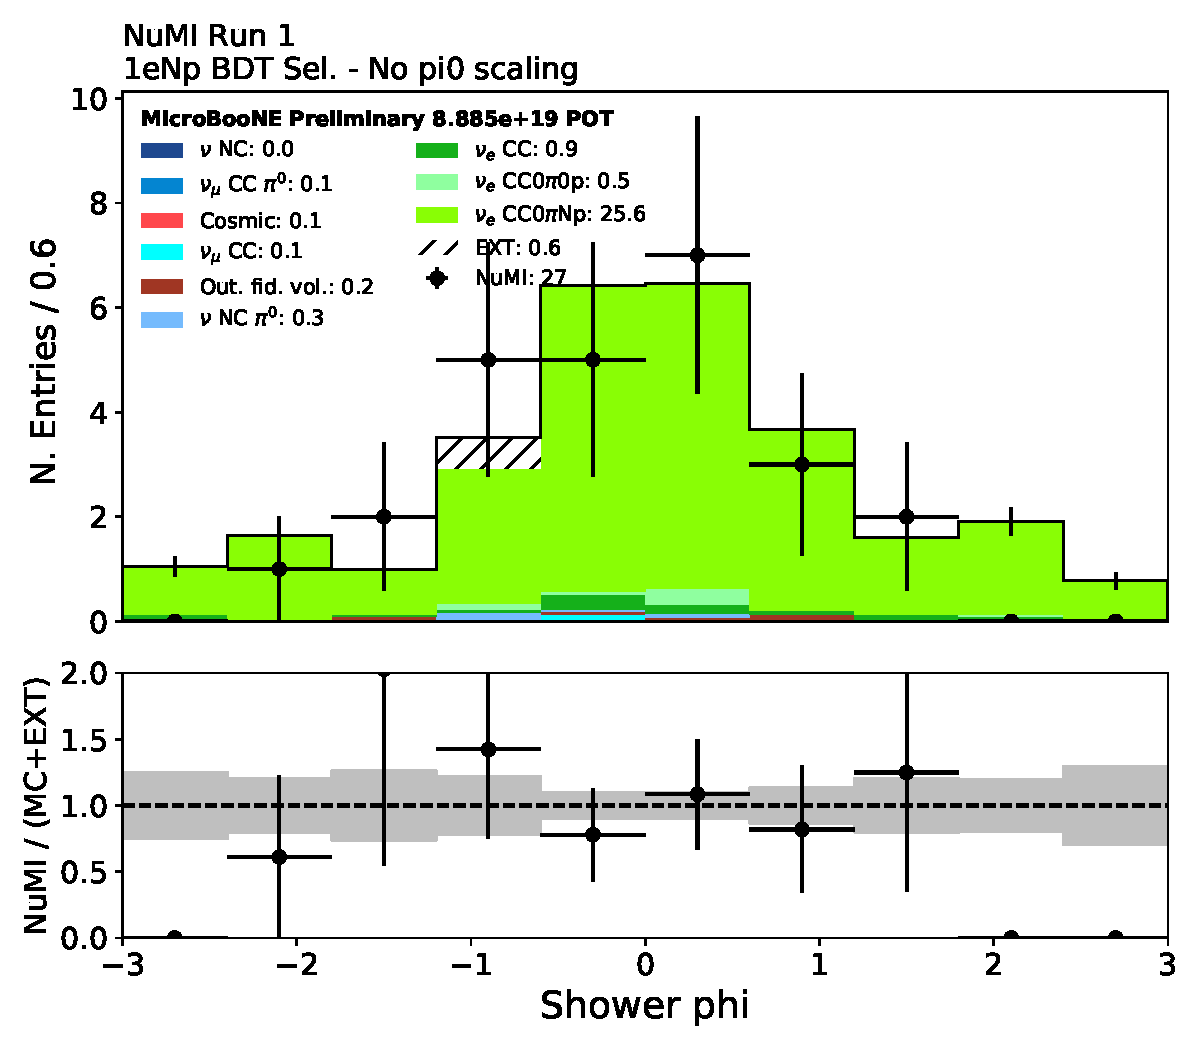
\includegraphics[width=1.0\textwidth]{Sidebands/Figures/NuMI/1eNp/BDTSel/shr_phi.pdf}
    \caption{}
    \end{subfigure}
    \caption{} 
    \label{fig:NuMI_1eNp_10}
\end{figure}

Figures~\ref{fig:NuMI_1eNp_1} shows the 6 events with energy lower than 500 MeV identified in the NuMI dataset by the \npsel final selection.


\begin{figure}[H]
    \begin{center}
    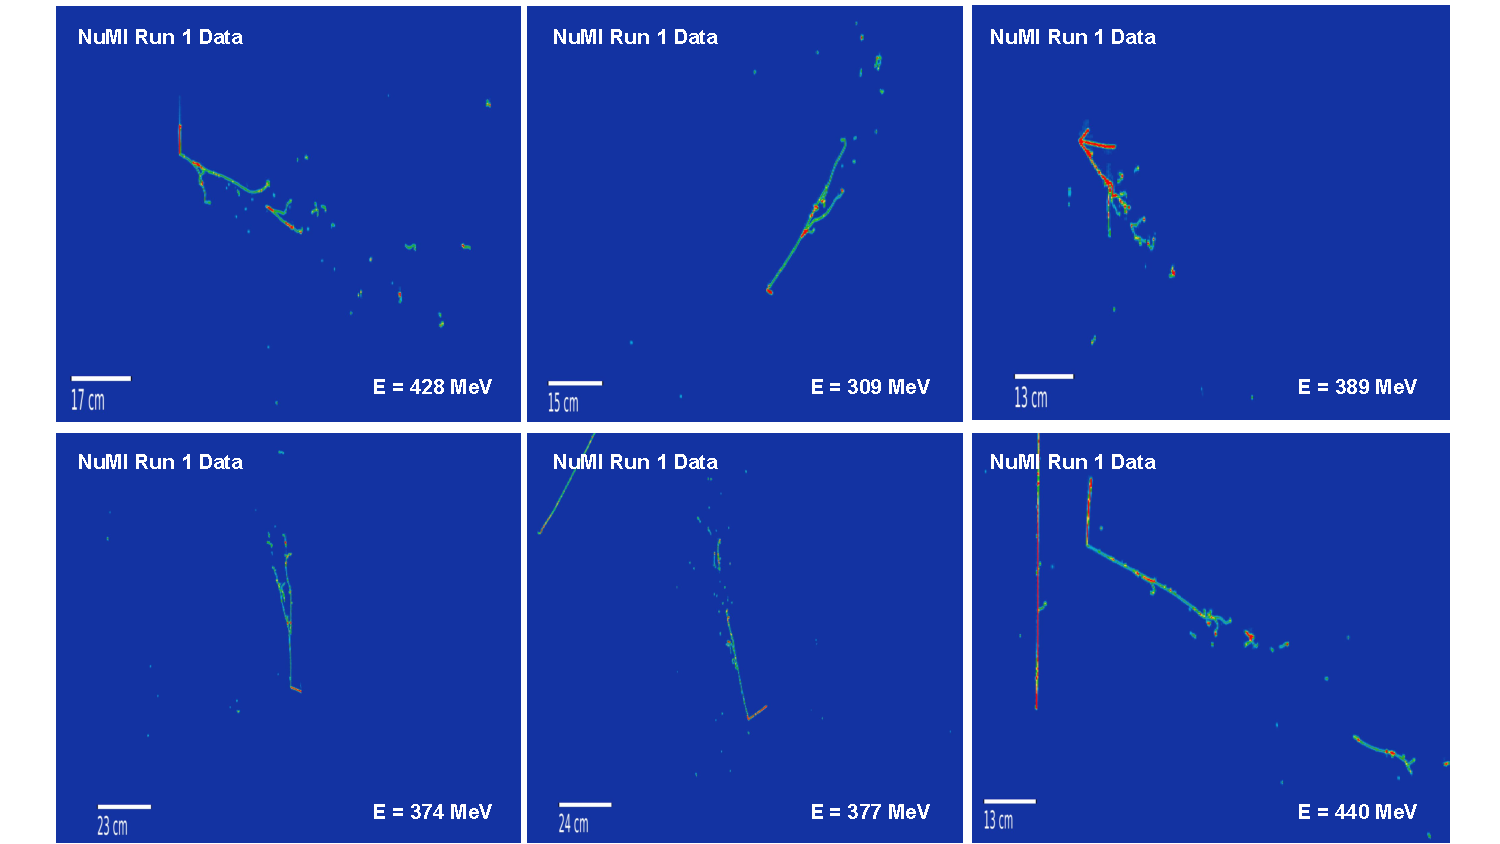
\includegraphics[width=\textwidth]{Sidebands/Figures/NuMI/1eNp/BDTSel/Evds.pdf}
    \caption{}
    \label{fig:NuMI_1eNp_11}
    \end{center}
\end{figure}

%\subsubsection{NuMI 1e0p0 Sideband/Elena}
%\subsubsection{NuMI $\pi^0$ Sideband/Elena}



